\documentclass[a4paper,12pt,times,print,index,custombib,custommargin]{PhDThesisPSnPDF}\usepackage[]{graphicx}\usepackage[]{color}
%% maxwidth is the original width if it is less than linewidth
%% otherwise use linewidth (to make sure the graphics do not exceed the margin)
\makeatletter
\def\maxwidth{ %
  \ifdim\Gin@nat@width>\linewidth
    \linewidth
  \else
    \Gin@nat@width
  \fi
}
\makeatother

\definecolor{fgcolor}{rgb}{0.345, 0.345, 0.345}
\newcommand{\hlnum}[1]{\textcolor[rgb]{0.686,0.059,0.569}{#1}}%
\newcommand{\hlstr}[1]{\textcolor[rgb]{0.192,0.494,0.8}{#1}}%
\newcommand{\hlcom}[1]{\textcolor[rgb]{0.678,0.584,0.686}{\textit{#1}}}%
\newcommand{\hlopt}[1]{\textcolor[rgb]{0,0,0}{#1}}%
\newcommand{\hlstd}[1]{\textcolor[rgb]{0.345,0.345,0.345}{#1}}%
\newcommand{\hlkwa}[1]{\textcolor[rgb]{0.161,0.373,0.58}{\textbf{#1}}}%
\newcommand{\hlkwb}[1]{\textcolor[rgb]{0.69,0.353,0.396}{#1}}%
\newcommand{\hlkwc}[1]{\textcolor[rgb]{0.333,0.667,0.333}{#1}}%
\newcommand{\hlkwd}[1]{\textcolor[rgb]{0.737,0.353,0.396}{\textbf{#1}}}%

\usepackage{framed}
\makeatletter
\newenvironment{kframe}{%
 \def\at@end@of@kframe{}%
 \ifinner\ifhmode%
  \def\at@end@of@kframe{\end{minipage}}%
  \begin{minipage}{\columnwidth}%
 \fi\fi%
 \def\FrameCommand##1{\hskip\@totalleftmargin \hskip-\fboxsep
 \colorbox{shadecolor}{##1}\hskip-\fboxsep
     % There is no \\@totalrightmargin, so:
     \hskip-\linewidth \hskip-\@totalleftmargin \hskip\columnwidth}%
 \MakeFramed {\advance\hsize-\width
   \@totalleftmargin\z@ \linewidth\hsize
   \@setminipage}}%
 {\par\unskip\endMakeFramed%
 \at@end@of@kframe}
\makeatother

\definecolor{shadecolor}{rgb}{.97, .97, .97}
\definecolor{messagecolor}{rgb}{0, 0, 0}
\definecolor{warningcolor}{rgb}{1, 0, 1}
\definecolor{errorcolor}{rgb}{1, 0, 0}
\newenvironment{knitrout}{}{} % an empty environment to be redefined in TeX

\usepackage{alltt}
%\documentclass[a4paper,12pt,times,numbered,print,index]{PhDThesisPSnPDF}

\usepackage{import}
%
% ******************************************************************************
% ****************************** Custom Margin *********************************

% Add `custommargin' in the document class options to use this section
% Set {innerside margin / outerside margin / topmargin / bottom margin}  and
% other page dimensions
\ifsetCustomMargin
  \RequirePackage[left=42mm,right=35mm,top=25mm,bottom=20mm]{geometry}
  \setFancyHdr % To apply fancy header after geometry package is loaded
\fi

% *****************************************************************************
% ******************* Fonts (like different typewriter fonts etc.)*************

% Add `customfont' in the document class option to use this section

\ifsetCustomFont
  % Set your custom font here and use `customfont' in options. Leave empty to
  % load computer modern font (default LaTeX font).
  \RequirePackage{helvet}
\fi

% *****************************************************************************
% **************************** Custom Packages ********************************
\usepackage{import}

%\usepackage{comment}

\usepackage{epigraph}

%% ---- package for formatting code with line numbers
\usepackage{fancyvrb} %% for verbatim text

\usepackage{ulem} % more underlining and other font effects

% ************************** Custom Floats **********************************
\usepackage{float}
\floatstyle{ruled}
\newfloat{cmd}{htb}{loc}[chapter]
\floatname{cmd}{Command}
% **** **** **** **** **** **** **** ****

%% ---- provides "\rowcolors" command
\usepackage[dvipsnames,table]{xcolor}

\usepackage{subcaption}

% ---- the following package call ensures that floats will not pass a section boundary ----
\usepackage[section]{placeins}
% ---- insert “\FloatBarrier” at places that floats should not move past, perhaps at every “\section”.

% ---- if I want to extract LaTeX formulas, for instance, 
% ---- to convert them into other picture formats from pdf
%\usepackage[active,tightpage]{preview}
% ---- use \begin{preiview} ... \end{preview}

\usepackage{relsize}
\renewcommand\RSsmallest{4pt}

%------ the following package can be used for Word Review function mimicking comments ----------%
\usepackage[textsize=tiny, textwidth=3cm, color=Dandelion, colorinlistoftodos]{todonotes} % specify ``disable'' to turn off all notes
\newcommand{\addcit}[1]{\todo[color=yellow!90,nolist]{#1}}
\newcommand{\comment}[1]{\todo[color=green!40,noline,nolist]{#1}} % the "comment" package also defines a command "\comment", so cannot use both
\newcommand{\longcomment}[1]{\todo[color=green!40,inline,nolist]{#1}}
\newcommand{\roger}[1]{\todo[color=blue!40]{Roger:\newline{}#1}}

%\ifsetDraft
%	\usepackage[textsize=tiny, textwidth=3cm, color=Dandelion, colorinlistoftodos]{todonotes} % specify ``disable'' to turn off all notes
%	\newcommand{\addcit}[1]{\todo[color=yellow!90,nolist]{#1}}
%	\newcommand{\comment}[1]{\todo[color=green!40,noline,nolist]{#1}}
%	\newcommand{\longcomment}[1]{\todo[color=green!40,inline,nolist]{#1}}
%	\newcommand{\roger}[1]{\todo[color=blue!40]{Roger:\newline{}#1}}
%\else
%	\newcommand{\addcit}[1]{}
%	\newcommand{\comment}[1]{}
%	\newcommand{\longcomment}[1]{}
%	\newcommand{\roger}[1]{}
%	\newcommand{\listoftodos}{}
%	\newcommand{\todo}{}
%\fi

%\usepackage{setspace}
%\newcommand{\note}[2][] {\todo[caption={#2}, #1] {\begin{spacing}{0.8}#2\end{spacing}}}

\usepackage{pdflscape}
\usepackage{lscape} % offers landscape environment, \begin{landscape}

% ---- for verbatim in captions. Usage: \cprotect\caption{...} ----
\usepackage{cprotect} 


% ************************* Algorithms and Pseudocode **************************

%\usepackage{algpseudocode}


% ********************Captions and Hyperreferencing / URL **********************

% Captions: This makes captions of figures use a boldfaced small font.
%\RequirePackage[small,bf]{caption}

\RequirePackage[labelsep=space,font=small,labelfont=bf,tableposition=top]{caption}
\DeclareCaptionLabelFormat{continued}{#1 #2 continued} 
\captionsetup[ContinuedFloat]{labelformat=continued}
\renewcommand{\figurename}{Fig.} %to support older versions of captions.sty
\usepackage{varioref}

\hypersetup{%
colorlinks=true,% 
citecolor=black,% 
linkcolor=black,
urlcolor=black% 
}



% *************************** Graphics and figures *****************************

%\usepackage{subfigure}

%\usepackage{rotating}
%\usepackage{wrapfig}

% Uncomment the following two lines to force Latex to place the figure.
% Use [H] when including graphics. Note 'H' instead of 'h'
%\usepackage{float}
%\restylefloat{figure}

% Subcaption package is also available in the sty folder you can use that by
% uncommenting the following line
% This is for people stuck with older versions of texlive
%\usepackage{sty/caption/subcaption}
\usepackage{subcaption}

% ********************************** Tables ************************************
\usepackage{booktabs} % For professional looking tables
\usepackage{multirow}
\usepackage{ctable}
\usepackage{colortbl}

%\usepackage{multicol}
%\usepackage{longtable}
%\usepackage{tabularx}


% ***************************** Math and SI Units ******************************

\usepackage{amsfonts}
\usepackage{amsmath}
\usepackage{amssymb}
\usepackage{siunitx} % use this package module for SI units


% ******************************* Line Spacing *********************************

% Choose linespacing as appropriate. Default is one-half line spacing as per the
% University guidelines

%\usepackage{setspace} % already loaded
% \doublespacing
% \onehalfspacing
% \singlespacing
% \setstretch{<baselinestretch>}

% e. g.:
%\begin{spacing}{1.2}
%\tableofcontents
%\listoffigures
%\listoftables
%\end{spacing}
\raggedbottom % leaves empty space at the bottom of pages if necessary


% ************************ Formatting / Footnote *******************************

% Don't break enumeration (etc.) across pages in an ugly manner (default 10000)
%\clubpenalty=500
%\widowpenalty=500

%\usepackage[perpage]{footmisc} %Range of footnote options

\renewcommand{\paragraph}[1]{ \textsc{#1} }


% *****************************************************************************
% *************************** Bibliography  and References ********************

%\usepackage{cleveref} %Referencing without need to explicitly state fig /table

% Add `custombib' in the document class option to use this section
\ifuseCustomBib
   \RequirePackage[square, sort, numbers, authoryear]{natbib} % CustomBib

% If you would like to use biblatex for your reference management, as opposed to the default `natbibpackage` pass the option `custombib` in the document class. Comment out the previous line to make sure you don't load the natbib package. Uncomment the following lines and specify the location of references.bib file

%\RequirePackage[backend=biber, style=numeric-comp, citestyle=numeric, sorting=nty, natbib=true]{biblatex}
%\bibliography{References/references} %Location of references.bib only for biblatex

\fi

% changes the default name `Bibliography` -> `References'
\renewcommand{\bibname}{References}


% *****************************************************************************
% *************** Changing the Visual Style of Chapter Headings ***************
% This section on visual style is from https://github.com/cambridge/thesis

% Uncomment the section below. Requires titlesec package.

%\RequirePackage{titlesec}
%\newcommand{\PreContentTitleFormat}{\titleformat{\chapter}[display]{\scshape\Large}
%{\Large\filleft{\chaptertitlename} \Huge\thechapter}
%{1ex}{}
%[\vspace{1ex}\titlerule]}
%\newcommand{\ContentTitleFormat}{\titleformat{\chapter}[display]{\scshape\huge}
%{\Large\filleft{\chaptertitlename} \Huge\thechapter}{1ex}
%{\titlerule\vspace{1ex}\filright}
%[\vspace{1ex}\titlerule]}
%\newcommand{\PostContentTitleFormat}{\PreContentTitleFormat}
%\PreContentTitleFormat


% ******************************************************************************
% ************************* User Defined Commands ******************************
% ******************************************************************************

% *********** To change the name of Table of Contents / LOF and LOT ************

%\renewcommand{\contentsname}{My Table of Contents}
%\renewcommand{\listfigurename}{My List of Figures}
%\renewcommand{\listtablename}{My List of Tables}

\newcommand{\marginal}[1]{
	\leavevmode\marginpar{\tiny\raggedright#1\par}}


% ********************** TOC depth and numbering depth *************************

\setcounter{secnumdepth}{2}
\setcounter{tocdepth}{2}


% ******************************* Nomenclature *********************************
 
% To change the name of the Nomenclature section, uncomment the following line

%\renewcommand{\nomname}{Symbols}


% ********************************* Appendix ***********************************

% The default value of both \appendixtocname and \appendixpagename is `Appendices'. These names can all be changed via:

%\renewcommand{\appendixtocname}{List of appendices}
%\renewcommand{\appendixname}{Appndx}

% ******************************** Draft Mode **********************************

% Uncomment to disable figures in `draftmode'
%\setkeys{Gin}{draft=true}  % set draft to false to enable figures in `draft'

% These options are active only during the draft mode
% Default text is "Draft"
%\SetDraftText{DRAFT}

% Default Watermark location is top. Location (top/bottom)
%\SetDraftWMPosition{bottom}

% Draft Version - default is v1.0
%\SetDraftVersion{v1.1}

% Draft Text grayscale value (should be between 0-black and 1-white)
% Default value is 0.75
%\SetDraftGrayScale{0.8}


%% Todo notes functionality
%% Uncomment the following lines to have todonotes.

%\ifsetDraft
%	\usepackage[colorinlistoftodos]{todonotes}
%	\newcommand{\mynote}[1]{\todo[author=kks32,size=\small,inline,color=green!40]{#1}}
%\else
%	\newcommand{\mynote}[1]{}
%	\newcommand{\listoftodos}{}
%\fi

% Example todo: \mynote{Hey! I have a note}

%%******************************** Glossary ***************************************************
\usepackage[toc,acronym]{glossaries}

% suppress page number list in glossary:
%\usepackage[nonumberlist]{glossaries}
%% *** \usepackage[toc,acronym]{glossaries}
% suppress page number list in glossary:
%\usepackage[nonumberlist]{glossaries}

%
% -- put the following code into a .latexmkrc file in the directory from where you run Latexmk --
%
%# add glossary generation to LATEXMK routine
%# ==========================================
%# taken from:
%# http://tex.stackexchange.com/questions/1226/how-to-make-latexmk-use-makeglossaries
%
%add_cus_dep('glo', 'gls', 0, 'run_makeglossaries');
%add_cus_dep('acn', 'acr', 0, 'run_makeglossaries');
%
%sub run_makeglossaries {
%  if ( $silent ) {
%    system "makeglossaries -q $_[0]";
%  }
%  else {
%    system "makeglossaries $_[0]";
%  };
%}
%
%push @generated_exts, 'glo', 'gls', 'glg';
%push @generated_exts, 'acn', 'acr', 'alg';
%$clean_ext .= ' %R.ist %R.xdy';

\makeglossaries

\renewcommand*{\glstextformat}[1]{\textsf{#1}}
%\renewcommand*{\glshyperlink}[1]{\textsf{#1}}

%--------------
% Glossary
%--------------
\newglossaryentry{fragment}{name=fragment, description={not a PCR duplicate. With paired reads from standard RAD (i. e. including random shearing of restriction fragments) typically identified by having different PE read sequences or different insert sizes after read mapping against a reference}}
\newglossaryentry{RAD tag}{name=RAD tag, description={genetic marker from RAD sequencing; the sequence up or downstream of a restriction site}}
\newglossaryentry{barcode}{name=barcode, description={short DNA sequence incorporated into adapter oligonucleotides that becomes part of the sequence read. Barcodes are used in order to be able to pool the DNA of different individuals, populations, treatments, etc. into one library that can be sequenced on one lane of an illumina flow cell}}
\newglossaryentry{index}{name=index, description={similar to barcode and serves the same purpose; generally incorporated into the centre of the adapter so that special sequencing run for the index is required} }
%\newglossaryentry{SbfI}{name=SbfI, description={restriction enzyme with the recognition sequence 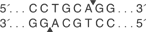
\includegraphics[scale=.5]{Sbf-I-cutsite_1_v1_000015}} }
\newglossaryentry{SbfI}{name=SbfI, description={restriction enzyme with the recognition sequence CCTGCA$\downarrow$GG} }
\newglossaryentry{XhoI}{name=XhoI, description={restriction enzyme with the recognition sequence C$\downarrow$TCGAG} }
\newglossaryentry{heterochromatin}{name=heterochromatin, description={Chromatin that remains in a highly condensed state throughout the cell cycle}}
\newglossaryentry{contig}{name=contig, description={longer consensus sequence derived from assembling smaller overlapping sequence reads}}
\newglossaryentry{linked RAD tag site}{name=linked RAD tag site, description={position in the reference sequence with at least one \gls{concordant} read pair on each side of a putative restriction site and the SE reads overlapping each other as expected from the restriction enzyme}}
\newglossaryentry{proper pair}{name=proper pair, description={read pair from illumina paired-end sequencing that got mapped to a reference in the correct orientation within a maximum expected distance from each other that is determined by the fragment size selection during the sequencing library preparation. Also called a \gls{concordant}ly mapping pair}}
\newglossaryentry{kmer}{name=kmer, description={subsequence with a specified length (k) of a longer sequence}}
\newglossaryentry{e-value}{name=Expect (E) value, description={The Expect value (E) is a parameter that describes the number of hits one can "expect" to see by chance when searching a database of a particular size}}
\newglossaryentry{read}{name=read, description={any sequence that comes out of the sequencer}}
\newglossaryentry{edit distance}{name=edit distance, description={minimum number of operations (one symbol insertion, deletion or substitution) required to change one string of symbols into another. Also known as \emph{Levenshtein distance}}}
\newglossaryentry{Ct}{name={C$_{t}$}, description={PCR cycle when a certain fluorescent threshold is reached}}
\newglossaryentry{mqs}{name={mapping quality score}, description={The mapping quality score \emph{Q} is the Phred transformation of the estimate of the probability \emph{p} that the reported mapping position does not correspond to the read's true point of origin: $Q = -10 \log_{10} p$. The way \emph{p} is estimated is different for each mapping programme, but in any case a mapping quality score \emph{Q} of 3 roughly corresponds to a mis-mapping probability \emph{p} of 0.5, i. e. the read has an estimated 50\% chance to have derived from a location other than the one reported}}
\newglossaryentry{discordant}{name=discordant, description={A read pair is called discordant if it aligns without the expected relative mate orientation (here: forward--reverse or reverse--forward) or outside the expected range of distances between mates. Note that \texttt{bowtie2} only calls discordant read pair mappings if both reads map \emph{uniquely}. Here, I am NOT adopting this requirement}}
\newglossaryentry{concordant}{name=concordant, description={A read pair is called concordant if it aligns with the expected relative mate orientation (here: forward--reverse or reverse--forward) and within the expected range of distances between mates. This is also called a \gls{proper pair}. The complement of \gls{discordant}}}
\newglossaryentry{Levenshtein distance}{name=Levenshtein distance, description={The Levenshtein distance is equal to the minimum number of operations (edits) required to transform one string into another. The allowed operations are single character insertions, deletions and substitutions. This is also known as edit distance.}}
\newglossaryentry{all pairs}{name={all pairs}, description={all the pairs of sequences below a given Levenshtein distance are identified during the graph construction phase}}
\newglossaryentry{transitive clusters}{name=transitive clusters, description={Two read clusters are merged if the distance of any pair of reads between the clusters is below threshold. After merging, the newly created cluster can contain read pairs with distance above the clustering threshold}}
\newglossaryentry{graph}{name=graph, description={A network of connected sequences. Two sequences are directly connected if they match with distance below a threshold. The distance is a measure of the strength of connection, aka "edge weight". Graphs can be stored as a list of pairs of sequences, with an optional edge weight. All graphs here should be "undirected cyclic graphs"}}
\newglossaryentry{Nmer}{name=\emph{N}mer, description={synonymous to kmer, unit, word; a subsequence of size \emph{N} that is overlapping or contiguous with the next subsequence of size \emph{N} and stored in a dictionnary (aka hash) for fast lookup}}
\newglossaryentry{population allele frequency}{name=population allele frequency, description={The population allele frequency is the (unknown) frequency of the allele in the entire population}}
\newglossaryentry{sample allele frequency}{name=sample allele frequency, description={The sample allele frequency is the frequency of the allele among the individuals in a specific sample}}
\newglossaryentry{connected component}{name=connected component, description={All nodes (here sequence reads) after all--pairs search (and before clustering!) that are directly connected by an edge or indirectly connected via several nodes belong to the same connected component} }

%----------------
% Acronyms
%----------------
\newacronym{snp}{SNP}{single nucleotide polymorphism}
\newacronym{rad}{RAD}{Restriction Site associated DNA}
\newacronym{pe}{PE}{paired-end}
\newacronym{se}{SE}{single-end}
\newacronym{bp}{bp}{base pair}
\newacronym{Mbp}{Mbp}{mega base pairs}
\newacronym{Gbp}{Gbp}{giga base pairs}
\newacronym{indel}{indel}{small sequence insertion or deletion polymorphism}
\newacronym{SAM}{SAM}{Sequence Alignment/Map format}
\newacronym{EST}{EST}{expressed sequence tag}
\newacronym{ddRAD}{ddRAD}{double digest RAD}
\newacronym{ML}{ML}{maximum likelihood}
\newacronym{SFS}{SFS}{site frequency spectrum}
\newacronym{HWE}{HWE}{Hardy Weinberg equilibrium}
\newacronym{CI}{CI}{confidence interval}
\newacronym{EM}{EM}{Expectation Maximisation}
\newacronym{DEM}{DEM}{digital elevation model}
%\usepackage[toc]{glossaries}
%\renewcommand*{\glstextformat}[1]{\textsf{#1}}
%
%\newglossaryentry{fragment}{name=fragment, description={not a PCR duplicate}}
%
%\newacronym{snp}{SNP}{single nucleotide polymorphism}

%% ******************************** SVG *************************************
%\newcommand{\executeiffilenewer}[3]{%
%	\ifnum\pdfstrcmp{\pdffilemoddate{#1}}%
%	{\pdffilemoddate{#2}}>0%
%	{\immediate\write18{#3}}\fi%
%}
%\newcommand{\includesvg}[1]{%
%	\executeiffilenewer{#1.svg}{#1.pdf}%
%	{./inkscape -z -D -f #1.svg %
%	--export-pdf=#1.pdf --export-latex}%
%	\import{./Figs/Inkscape_Graphics}{#1.pdf_tex}%
%}


%
%%******************************** Glossary *********************************************
% *** \usepackage[toc,acronym]{glossaries}
% suppress page number list in glossary:
%\usepackage[nonumberlist]{glossaries}

%
% -- put the following code into a .latexmkrc file in the directory from where you run Latexmk --
%
%# add glossary generation to LATEXMK routine
%# ==========================================
%# taken from:
%# http://tex.stackexchange.com/questions/1226/how-to-make-latexmk-use-makeglossaries
%
%add_cus_dep('glo', 'gls', 0, 'run_makeglossaries');
%add_cus_dep('acn', 'acr', 0, 'run_makeglossaries');
%
%sub run_makeglossaries {
%  if ( $silent ) {
%    system "makeglossaries -q $_[0]";
%  }
%  else {
%    system "makeglossaries $_[0]";
%  };
%}
%
%push @generated_exts, 'glo', 'gls', 'glg';
%push @generated_exts, 'acn', 'acr', 'alg';
%$clean_ext .= ' %R.ist %R.xdy';

\makeglossaries

\renewcommand*{\glstextformat}[1]{\textsf{#1}}
%\renewcommand*{\glshyperlink}[1]{\textsf{#1}}

%--------------
% Glossary
%--------------
\newglossaryentry{fragment}{name=fragment, description={not a PCR duplicate. With paired reads from standard RAD (i. e. including random shearing of restriction fragments) typically identified by having different PE read sequences or different insert sizes after read mapping against a reference}}
\newglossaryentry{RAD tag}{name=RAD tag, description={genetic marker from RAD sequencing; the sequence up or downstream of a restriction site}}
\newglossaryentry{barcode}{name=barcode, description={short DNA sequence incorporated into adapter oligonucleotides that becomes part of the sequence read. Barcodes are used in order to be able to pool the DNA of different individuals, populations, treatments, etc. into one library that can be sequenced on one lane of an illumina flow cell}}
\newglossaryentry{index}{name=index, description={similar to barcode and serves the same purpose; generally incorporated into the centre of the adapter so that special sequencing run for the index is required} }
%\newglossaryentry{SbfI}{name=SbfI, description={restriction enzyme with the recognition sequence 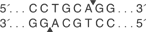
\includegraphics[scale=.5]{Sbf-I-cutsite_1_v1_000015}} }
\newglossaryentry{SbfI}{name=SbfI, description={restriction enzyme with the recognition sequence CCTGCA$\downarrow$GG} }
\newglossaryentry{XhoI}{name=XhoI, description={restriction enzyme with the recognition sequence C$\downarrow$TCGAG} }
\newglossaryentry{heterochromatin}{name=heterochromatin, description={Chromatin that remains in a highly condensed state throughout the cell cycle}}
\newglossaryentry{contig}{name=contig, description={longer consensus sequence derived from assembling smaller overlapping sequence reads}}
\newglossaryentry{linked RAD tag site}{name=linked RAD tag site, description={position in the reference sequence with at least one \gls{concordant} read pair on each side of a putative restriction site and the SE reads overlapping each other as expected from the restriction enzyme}}
\newglossaryentry{proper pair}{name=proper pair, description={read pair from illumina paired-end sequencing that got mapped to a reference in the correct orientation within a maximum expected distance from each other that is determined by the fragment size selection during the sequencing library preparation. Also called a \gls{concordant}ly mapping pair}}
\newglossaryentry{kmer}{name=kmer, description={subsequence with a specified length (k) of a longer sequence}}
\newglossaryentry{e-value}{name=Expect (E) value, description={The Expect value (E) is a parameter that describes the number of hits one can "expect" to see by chance when searching a database of a particular size}}
\newglossaryentry{read}{name=read, description={any sequence that comes out of the sequencer}}
\newglossaryentry{edit distance}{name=edit distance, description={minimum number of operations (one symbol insertion, deletion or substitution) required to change one string of symbols into another. Also known as \emph{Levenshtein distance}}}
\newglossaryentry{Ct}{name={C$_{t}$}, description={PCR cycle when a certain fluorescent threshold is reached}}
\newglossaryentry{mqs}{name={mapping quality score}, description={The mapping quality score \emph{Q} is the Phred transformation of the estimate of the probability \emph{p} that the reported mapping position does not correspond to the read's true point of origin: $Q = -10 \log_{10} p$. The way \emph{p} is estimated is different for each mapping programme, but in any case a mapping quality score \emph{Q} of 3 roughly corresponds to a mis-mapping probability \emph{p} of 0.5, i. e. the read has an estimated 50\% chance to have derived from a location other than the one reported}}
\newglossaryentry{discordant}{name=discordant, description={A read pair is called discordant if it aligns without the expected relative mate orientation (here: forward--reverse or reverse--forward) or outside the expected range of distances between mates. Note that \texttt{bowtie2} only calls discordant read pair mappings if both reads map \emph{uniquely}. Here, I am NOT adopting this requirement}}
\newglossaryentry{concordant}{name=concordant, description={A read pair is called concordant if it aligns with the expected relative mate orientation (here: forward--reverse or reverse--forward) and within the expected range of distances between mates. This is also called a \gls{proper pair}. The complement of \gls{discordant}}}
\newglossaryentry{Levenshtein distance}{name=Levenshtein distance, description={The Levenshtein distance is equal to the minimum number of operations (edits) required to transform one string into another. The allowed operations are single character insertions, deletions and substitutions. This is also known as edit distance.}}
\newglossaryentry{all pairs}{name={all pairs}, description={all the pairs of sequences below a given Levenshtein distance are identified during the graph construction phase}}
\newglossaryentry{transitive clusters}{name=transitive clusters, description={Two read clusters are merged if the distance of any pair of reads between the clusters is below threshold. After merging, the newly created cluster can contain read pairs with distance above the clustering threshold}}
\newglossaryentry{graph}{name=graph, description={A network of connected sequences. Two sequences are directly connected if they match with distance below a threshold. The distance is a measure of the strength of connection, aka "edge weight". Graphs can be stored as a list of pairs of sequences, with an optional edge weight. All graphs here should be "undirected cyclic graphs"}}
\newglossaryentry{Nmer}{name=\emph{N}mer, description={synonymous to kmer, unit, word; a subsequence of size \emph{N} that is overlapping or contiguous with the next subsequence of size \emph{N} and stored in a dictionnary (aka hash) for fast lookup}}
\newglossaryentry{population allele frequency}{name=population allele frequency, description={The population allele frequency is the (unknown) frequency of the allele in the entire population}}
\newglossaryentry{sample allele frequency}{name=sample allele frequency, description={The sample allele frequency is the frequency of the allele among the individuals in a specific sample}}
\newglossaryentry{connected component}{name=connected component, description={All nodes (here sequence reads) after all--pairs search (and before clustering!) that are directly connected by an edge or indirectly connected via several nodes belong to the same connected component} }

%----------------
% Acronyms
%----------------
\newacronym{snp}{SNP}{single nucleotide polymorphism}
\newacronym{rad}{RAD}{Restriction Site associated DNA}
\newacronym{pe}{PE}{paired-end}
\newacronym{se}{SE}{single-end}
\newacronym{bp}{bp}{base pair}
\newacronym{Mbp}{Mbp}{mega base pairs}
\newacronym{Gbp}{Gbp}{giga base pairs}
\newacronym{indel}{indel}{small sequence insertion or deletion polymorphism}
\newacronym{SAM}{SAM}{Sequence Alignment/Map format}
\newacronym{EST}{EST}{expressed sequence tag}
\newacronym{ddRAD}{ddRAD}{double digest RAD}
\newacronym{ML}{ML}{maximum likelihood}
\newacronym{SFS}{SFS}{site frequency spectrum}
\newacronym{HWE}{HWE}{Hardy Weinberg equilibrium}
\newacronym{CI}{CI}{confidence interval}
\newacronym{EM}{EM}{Expectation Maximisation}
\newacronym{DEM}{DEM}{digital elevation model}

%%%%%% -- KNITR SETUP -- %%%%%%%%%%

%%%%%%%%%%%%%%%%%%%%%%%%%%
\IfFileExists{upquote.sty}{\usepackage{upquote}}{}
\begin{document}
%
\tableofcontents
%
%\listoffigures

%\listof{cmd}{List of commands}

%\todototoc
\listoftodos

\printglossaries



% **************************** Define Graphics Path **************************
%% Note, every path needs to end with a "/" !!!
\ifpdf
    \graphicspath{
    {./Figs/Raster/}
    {./Figs/PDF/}
    {./Figs/}
    {/Users/Claudius/Documents/PhD/THESIS/kks32/LaTeX/Data_analysis/reference-mapping/figure/}
    {/Users/Claudius/Documents/PhD/THESIS/kks32/LaTeX/3_Chapter/Figs/}
    }
\else
    \graphicspath{ 
%    {./Figs/Vector/}
%    {./Figs/}
    {/Users/Claudius/Documents/PhD/THESIS/kks32/LaTeX/3_Chapter/Figs/}
    }
\fi


% ************************************************************************************

%
%
%
\chapter{Testing incomplete digestion}
%
%
%

%\epigraph{Nothing in biology makes sense, except in the light of evolution}{Theodosius Dobzhansky}
%
%\epigraph{\dots it occurred to me to ask the question, Why do some die and some live? And the answer was clearly, that on the whole the best fitted live. [\dots] Then it suddenly flashed upon me that this self-acting process would necessarily improve the race, because in every generation the inferior would inevitably be killed off and the superior would remain-that is, the fittest would survive \dots}{Alfred Russel Wallace}
% other sources of epigraphs: mindfulness book, Ada Lovelace

\epigraph{
Bonzai: Are you as successful as you would like to be?

Zappa: I would say that the basic characteristic of my life is failure. 
If there is one thing that I excel at, it's failure -- I manage to fail at 100 percent of the things that I do. 
Since most of the things that I set out to do are theoretically impossible, it's very easy to fail. 
I've learned to live with it. 
In terms of machinery and personnel, there never seems to be enough to get things done exactly right.
}{interview with Frank Zappa, 1985}

% ------------------------------------------------------------------------------------------------
%<<set working directory, echo=FALSE, cache=TRUE>>=
%@
% ------------------------------------------------------------------------------------------------

% --------------------------------
\section{Introduction}
% --------------------------------
%\begin{itemize}
%\item Why do I need many markers ?
%\item Do I need genotypes ?
%\item What about pooled data ?
%\item What other types of population genetic analyses benefit from many markers for many individuals ?
%\item non-model organisms
%\item Do I need to explain why certain types of population genetic analyses need many markers and many individuals?
%\item Which analyses require genotypes ?
%\end{itemize}
%
%\begin{itemize}
%\item Various population genetic analyses require many markers from many individuals -- first paragraph
%\item various technical problems with RAD, literature, examples, not in detail, genotype calls necessary for some analyses
%\item among those technical problems are incomplete digestion, religation, low temlate amonbunt
%\item got RAD data set with initial intention of doing hybrid zone analysis, illustrate some of these problems
%\end{itemize}

%%% -----------------------------------------------------------------------------------------------------------------------------
%\paragraph{Various population genetic analyses require many markers from many individuals}
%%% -----------------------------------------------------------------------------------------------------------------------------

%Many population genetic analyses require many genetic markers from a large number of individuals for precise and reliable inferences of population genetic parameters \citep{Pool2010,Luikart2003}. Genome-wide association studies, for instance, have the power, despite correction for multiple testing, to detect marker--trait associations in a genome-wide scan for associations with millions of markers \citep{Risch1996}. \todo{add more empirical examples} \comment{more empirical examples of studies using many markers, first from model organisms (mice), then later with RAD in non-model organisms} \addcit{\cite{Evans2014}, \cite{Catchen2013}, \cite{Merz2013}} 
%\\




\cite{Altshuler2000} were the first to use reduced-representation sequencing libraries from genomic restriction fragments for SNP discovery (now widely called \gls{rad}). After the introduction of massively parallel sequencing technologies, these were further developed for population allele frequency and genotype estimation \citep{Baird2008,VanTassell2008,Andolfatto2011,Elshire2011,Davey2011}.  By sequencing only the ends of restriction fragments, \gls{rad} creates sequencing libraries with reduced complexity as compared to whole-genome shotgun sequencing, thus subsampling the genome at homologous locations to identify and type SNPs evenly throughout the genome and increasing \gls{read} coverage for a given sequenced site. It is therefore a cost--effective alternative to whole genome shotgun sequencing of random loci. It is also superior to microsatellites, AFPL or EST markers since it can be used with study organisms without genome sequence information and allows genome-wide discovery of co--dominant genetic markers and their genotyping in one go \citep{Davey2011}. If template molecules for sequencing are labelled with different \glspl{barcode} from ligated adapter oligonucleotides, then individual or population samples can be pooled during sequence library preparation and sequenced together in the same parallel sequencing run. restriction enzyme--based genotyping by sequencing (GBS) technique \\
the regions of the genome that flank the recognition sites of restriction enzymes \\
reduced rep- resentation libraries (RRL) have been used to subsample genomes in a repeatable manner



%\begin{itemize}
%\item QTL, association mapping \\
%no genotypes, only allele frequencies are necessary for association studies \cite{Lander1994}. Association studies test whether a particular \emph{allele} at a locus occurs at significantly higher frequency among affected than unaffected individuals. \\
%Association analysis of F2 or backcross individuals from experimental crosses or linkage analysis from wild pedigrees capture only few recombinations that allow for a disassociation of weakly linked markers to a causative allele. Association mapping within wild populations, on the other hand, uses many historical recombinations from wild populations and thus allows in principle a much finer scale of mapping of loci affecting variation in the focal trait. Thus, genome-wide association studies can benefit from a high density of genetic markers across the genome. 
%\item hybrid zone analyses \cite{Barton1979}, \cite{Gompert2009}
%\item population structure and demographic history \cite{Pool2009}, 
%\item estimation of selection, recombination rate , mutation \cite{Lynch2008}, \cite{Fumagalli2013a}
%\end{itemize}
%
%The prgramme \texttt{structure} \cite{Pritchard2000} uses the genotypic correlations (i. e. LD) among physically unlinked markers to infer population structure and the origin of sampled individuals within subpopulations.

%Developing hundreds or even thousands of polymorphic microsatellite markers is costly and time-consuming for species without a close relative with a sequenced genome or collection of known polymorphic microsatellite markers \cite{Dawson2010}. Once developed, the genotyping of many microsatellite markers in many individuals is again costly and time-consuming.

%\begin{itemize}
%\item \cite{Davey2011}, 
%\item \cite{Andrews2014a}, 
%\item \cite{Andrews2014}, 
%\item \cite{Andrews2014a}, 
%\item \cite{Puritz2014}, 
%\item \cite{Davey2010a}, 
%\end{itemize}


%%% -----------------------------------------------------------------------------------------------------------------------------
%\paragraph{Various technical problems with RAD}
%%% -----------------------------------------------------------------------------------------------------------------------------
RAD markers, however, pose several challenges to unbiased estimation of population genetic parameters \citep{Ilut2014,Gautier2012,Davey2012,Luca2011,Arnold2013}. Among these are null--alleles from polymorphisms in the restriction recognition sequence. \todo{expand} \addcit{\cite{Mastretta-Yanes2015}} \comment{show that my intended analyses pose common problems in population and quantitative genetics which require many markers for many individuals} \comment{explain that analyses that require genotype calls need much better quality data than analyses that only require estimation of population allele frequency} \comment{Zac Gompert's Bayesian approach to genotype calling}
%
%genotype calls necessary for some analyses: 
%
%\begin{itemize}
%\item genomic clines \cite{Gompert2010a}
%\item QTL, 
%\item LD (gametic phase disequilibrium) estimates, linkage patterns, e. g. admixture linkage disequilibrium to estimate ancestry along chromosomes, genotypes and phasing of alleles into haplotypes, codominant markers necessary, admixture mapping to benefit from temporarily increased LD when marker density is limited
%\end{itemize}
%
%higher per individual coverage needed for studies that require genotypes as compared to studies requiring only population allele frequencies \cite{Buerkle2012} \\
%issue of low coverage \\
%ascertainment bias ? \\
%\cite{Davey2012}, \cite{Gautier2012}, \cite{Luca2011}, \cite{Arnold2013}

%%% -----------------------------------------------------------------------------------------------------------------------------
%\paragraph{RAD data set that illustrates some of these problems}
%%% -----------------------------------------------------------------------------------------------------------------------------
Here I am using two different types of \gls{rad} data sets\footnote{that were initially created with the intention of doing a hybrid zone analysis} to investigate three issues that can occur during the preparation of \gls{rad} libraries and that can lead to unusually low overall coverage and an extreme variation in coverage among loci and individuals: incomplete digestion, genomic re--ligation and low genomic template amount. I am showing bioinformatic analyses that can detect or at least distinguish among these issues post--sequencing and I suggest suitable measures for the library preparation that can mitigate their impact. 



%% ---------------------------------------------------
\subsection{Two different types of RAD}
%% ---------------------------------------------------

%\begin{itemize}
%\item why not microsats, AFLP \\
%due to the large number of possible alleles, microsats can be very polymorphic, therefore have heterozygosity and thus highly informative to detect recombination, although homoplasy could be an issue, paternity inference, population structure, gene flow, linkage mapping, the isolation and development of microsatellites is a skilled and time- consuming task that can take weeks or months to complete and is therefore costly to perform. Developing hundreds or even thousands of microsats and then scoring them in hundreds of individuals is prohibitive in time and financial costs. Mutation mode and mutation rates are generally not known for microsats. There are many more SNP's than microsats in any genome
%\item review marker techniques ?
%\end{itemize}

\gls{rad}, aka RADseq, is the high-throughput sequencing of restriction fragment ends (figure \ref{RAD_protocol_overview}). It requires no prior genome sequence information. Only genome size and GC content are required to estimate the required number of \glspl{read} for a certain target coverage. 
RADseq can yield co-dominant \gls{snp} markers in \glspl{RAD tag}, dominant presence/absence markers when the restriction site sequence is polymorphic or short \gls{indel} polymorphisms when the clustering algorithm allows for them. Additionally, when doing \gls{pe} sequencing, a \gls{pe} contig can be assembled for a given \gls{RAD tag} (figure \ref{RAD_protocol_overview}).
Given enough coverage and when using adapters with barcode sequences, individual genotypes can be scored.

Since this \emph{standard} version of \gls{rad} according to \cite{Baird2008} generates tags around every restriction site (figure \ref{RAD_protocol_overview}), it allows for only limited complexity reduction. Further complexity reduction can be achieved by skipping the step of shearing the restriction fragments and instead size selecting a range of restriction fragments that have the right size for the sequencing platform \citep{Andolfatto2011}. Further fine tuning of fragment number can be achieved when digesting DNA with two enzymes, so-called double-digest \gls{rad} (figure \ref{ddRAD_protocol_overview}) \citep{Peterson2012}.
% ---- add glossary entrywithout generating text ----
\glsadd[]{barcode} % allows to use \glshyperlink in captions

\begin{figure}
\centering
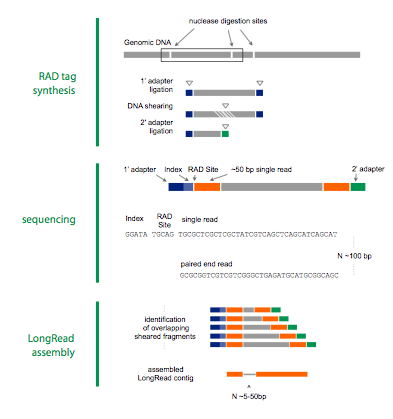
\includegraphics[width=.7\textwidth]{RADprotocolOverview}
\caption[Overview of the RAD marker technique.]{Overview of the \gls{rad} marker technique. (1) One restriction enzyme is used to digest genomic DNA. The first illumina adapter (P1), containing a different \glshyperlink[\textsf{barcode}]{barcode} (here called \gls{index}) sequence for each individual, is then ligated to the restriction fragments. The restriction fragments are then sheared, usually by high-frequency sonication, into a fragment size range that is suitable for illumina sequencing, which is selected on an agarose gel. After ligation of the second illumina adapter (P2), fragments with at least one P1 adapter are enriched by selective PCR. (2) The \gls{se} reads start with a barcode sequence, followed by the remainder of the restriction site. Only relatively short sequences (tags) are generated from the ends of the fragments. (3) Due to random shearing of restriction fragments, the \gls{pe} reads start at variable genomic distance from the restriction site (unless they are PCR duplicates) and thus can be assembled into short \gls{pe} contigs, depending on the size range selected on the gel. Taken from \cite{Atwood2011}. }
\label{RAD_protocol_overview}
\end{figure}
%
\begin{figure}
%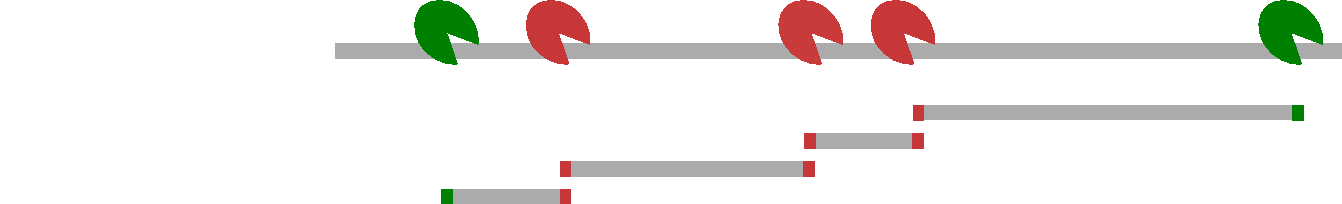
\includegraphics[width=\textwidth]{/Users/Claudius/Documents/PhD/sRAD/RAD_sketches/RAD_sketches}\\
%\includegraphics[width=\textwidth]{/Users/Claudius/Documents/PhD/sRAD/RAD_sketches/RAD_sketches_1}\\
\def\svgwidth{.9\textwidth}
\subimport{/Users/Claudius/Documents/PhD/THESIS/kks32/LaTeX/3_Chapter/Figs/Inkscape_Graphics/}{ddRAD_overview_1.pdf_tex}\\ 
\def\svgwidth{\textwidth}
\subimport{/Users/Claudius/Documents/PhD/THESIS/kks32/LaTeX/3_Chapter/Figs/Inkscape_Graphics/}{ddRAD_overview_2.pdf_tex}\\
\def\svgwidth{.9\textwidth}
\subimport{/Users/Claudius/Documents/PhD/THESIS/kks32/LaTeX/3_Chapter/Figs/Inkscape_Graphics/}{ddRAD_overview_3.pdf_tex}\\
\def\svgwidth{.9\textwidth}
\subimport{/Users/Claudius/Documents/PhD/THESIS/kks32/LaTeX/3_Chapter/Figs/Inkscape_Graphics/}{ddRAD_overview_4.pdf_tex}\\
\def\svgwidth{.9\textwidth}
\subimport{/Users/Claudius/Documents/PhD/THESIS/kks32/LaTeX/3_Chapter/Figs/Inkscape_Graphics/}{ddRAD_overview_5.pdf_tex}
\caption[Double-digest RAD protocol overview.]{Double-digest RAD protocol overview.}
\label{ddRAD_protocol_overview}
\end{figure}

\begin{figure}[t]
\ContinuedFloat
\caption[]{Genomic DNA is first digested by two different restriction enzymes (red and green). Illumina adapters (P1 and P2) are then ligated to the restriction fragments. The P2 adapter is a so-called divergent-Y adapter that, if anything, only contains the reverse-complement of the backward PCR primer binding site needed during the selective PCR step (see figure \ref{adapter_outline}). Restriction fragments are then size-selected on a gel. Here, in contrast to the standard RAD protocol (see fig. \ref{RAD_protocol_overview}), gel size selection selects which markers get into the final sequencing library. The selective PCR step enriches the library for fragments with at least one P1 adapter ligated to it. Bridge-amplification on the Illumina flow cell requires a P1 and a P2 adapter. Illumina paired-end sequencing results in two RAD tags per fragment that can be assembled and used for SNP and indel calling.}
\end{figure}


%% ------------------------------------
\subsection{The Problem}
%% ------------------------------------

A standard RAD library with the restriction enzyme \gls{SbfI} was prepared according to the protocol of Paul Etter, University of Oregon \citep{Baird2008}. The RAD library contained DNA from 36 grasshoppers sampled from the two distal populations ("Aunat" and "Greixer") of a transect through the \textit{Chorthippus parallelus / erythropus} hybrid zone in the Pyrenees between France and Spain \citep{Hewitt1987}. The RAD library was sequenced on an Illumina GAIIx and the resulting 46 \gls{bp}  long reads\footnote{after removing the barcode sequence} assembled with the programme suite \texttt{stacks} \citep{Catchen2011}.

Figure \ref{Big_Data:freq_dist_of_genotype_calls} shows the frequency distribution of loci -- reconstructed by \texttt{stacks} version 0.998 \todo{explain how \texttt{stacks} clusters reads and how it calls genotypes} -- over the number of individuals that have a genotype called for that locus. \texttt{Stacks} was run with a minimum allele coverage of 3 per individual and a maximum number of mismatches between alleles of 2 for merging alleles into loci within individuals as well as assembling a catalog of loci for the whole sample of 36 grasshoppers (further details can be looked up on the \href{http://creskolab.uoregon.edu/stacks/param_tut.php}{\texttt{stacks}} home page). About 50\% of the 379,720 unfiltered reconstructed loci have a genotype call in only one or two of the 36 individuals. About 170,000 RAD markers were expected from this library (see section \ref{ch:RAD_marker_number}) assuming a genome size of 12 giga \glspl{bp} (see section \ref{ch:Genome_size}).

%\begin{figure}
%\centering
%<<freq dist of genotype calls Big Data, echo=FALSE, out.width='.9\\linewidth', cache=TRUE>>=
%@
%\caption{Frequency distribution of loci, reconstructed by \texttt{stacks} (i. e. so-called "catalog stacks"), over the number of individuals in which they have a genotype call.}
%\label{Big_Data:freq_dist_of_genotype_calls}
%\end{figure}

Figure \ref{ddRAD:freq_dist_of_genotype_calls} shows the frequency distribution of reconstructed loci over the number of individuals for which they have a genotype called for the data of an \gls{SbfI}$+$\gls{XhoI} double-digest RAD library. The \gls{se} and \gls{pe} \glspl{RAD tag} have been merged into a 196 \gls{bp} long tag\footnote{including 11 bp remainders of restriction sites} before the assembly with \texttt{stacks}. \texttt{Stacks} was run with a minimum allele depth of 3 and maximum mismatch distance of 6 for merging alleles into read stacks within individuals as well as assembling a catalog of stacks (i. e. putative loci) from the individual stacks of all 36 grasshoppers (plus 2 technical replicates). Of the 156,532 putative loci that \texttt{stacks} had assembled, 51\% can only be found in one individual and only 3.5\% can be found in 20 or more individuals. Note that these numbers are from the raw output of \texttt{stacks} and do not include credibility filtering of putative loci and genotype calls. Around 16,000 RAD markers were expected from this double-digest RAD library (see equation \ref{eq:exp_number_ddRAD_loci} in section \ref{ch:RAD_marker_number}).
%
%\begin{figure}
%\centering
%<<freq dist of genotype calls SbfI-XhoI, echo=FALSE, out.width='.9\\linewidth', cache=TRUE>>=
%@
%\caption{Frequency distribution of catalog tags over the number of individuals in which they have a genotype call.}
%\label{ddRAD:freq_dist_of_genotype_calls}
%\end{figure}
%
\begin{figure}
\centering
\begin{subfigure}[t]{.495\textwidth}
\begin{knitrout}
\definecolor{shadecolor}{rgb}{0.969, 0.969, 0.969}\color{fgcolor}

{\centering \includegraphics[width=.9\linewidth]{figure/freq_dist_of_genotype_calls_Big_Data-1} 

}



\end{knitrout}
\caption{}
\label{Big_Data:freq_dist_of_genotype_calls}
\end{subfigure}
\hfill
\begin{subfigure}[t]{.495\textwidth}
\begin{knitrout}
\definecolor{shadecolor}{rgb}{0.969, 0.969, 0.969}\color{fgcolor}

{\centering \includegraphics[width=.9\linewidth]{figure/freq_dist_of_genotype_calls_SbfI-XhoI-1} 

}



\end{knitrout}
\caption{}
\label{ddRAD:freq_dist_of_genotype_calls}
\end{subfigure}
\caption{Frequency distribution of loci, reconstructed by \texttt{stacks} (i. e. so-called "catalog stacks"), over the number of individuals in which they have a genotype call.}
\label{freq_dist_of_genotype_calls}
\end{figure}

In the standard SbfI RAD data set, there are 5,014 \gls{se} reads and 25,268 \gls{pe} reads that apparently contain \gls{SbfI} recognition sites within them (30,282 in total)\footnote{counted with \texttt{grep -c}}. I searched in 88,734,712 quality filtered reads altogether. That is, 0.034\% of quality filtered reads contain an SbfI recognition site. Figure \ref{SbfI_frequency_dist_per_ind} shows the frequency distributions of SbfI sites in SE and PE reads for all 36 individuals separately (for further description see section \ref{site_frequency_distributions}). Obviously, if SbfI restriction and following P1 adapter ligation were 100\% efficient, there should be no SbfI recognition sequences in either SE or PE reads. 
%
\begin{figure}[htb]
\centering
\begin{knitrout}
\definecolor{shadecolor}{rgb}{0.969, 0.969, 0.969}\color{fgcolor}

{\centering 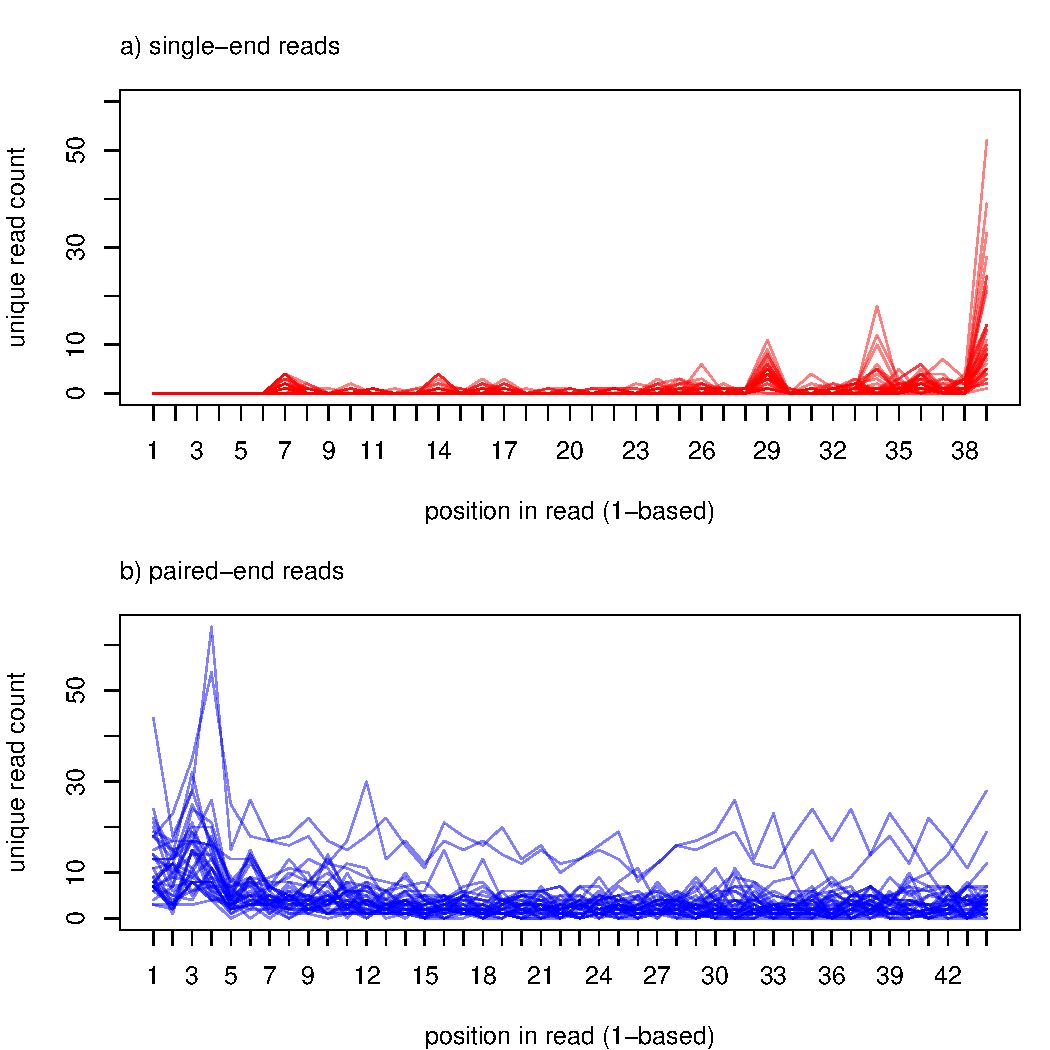
\includegraphics[width=.8\linewidth]{figure/SbfI_frequency_dist__per_ind_-1} 

}



\end{knitrout}
\caption{SbfI site frequency distributions across (a) SE and (b) PE reads for each of the 36 individuals in the standard RAD data set.}
\label{SbfI_frequency_dist_per_ind}
\end{figure}
%
Could this pattern be an indication that SbfI restriction during the library preparation was incomplete? If so, could there be a systematic variation between individuals in the completeness of restriction at individual SbfI sites that could lead to many loci only being detected in a few individuals as shown in figure \ref{freq_dist_of_genotype_calls}?
In the following I will investigate the potential role of incomplete restriction enzyme digestion \comment{not just incomplete digestion, also religation and low starting DNA amount} during the sequencing library preparation on the distribution of read coverage over \glspl{RAD tag} and on the resulting detection probability of RAD tags as shown in figure \ref{freq_dist_of_genotype_calls}.  


%% ---------------------------------------------------
\FloatBarrier
\section{Results and Discussion}
%% ---------------------------------------------------

%% ----------------------------------------------------------------
\FloatBarrier
\subsection{Assembling pairs of PE read contigs}
%% ----------------------------------------------------------------

Incomplete digestion for a specific SbfI site could in principle be tested with a PCR (or even quantified with \textit{q}PCR) across this site before and after digestion \citep{Luca2011}. However, no close reference sequence was available for PCR primer design at the time of this analysis\footnote{April 2014}. For a given \gls{RAD tag} from a standard RAD library, the PE reads can be used to assemble them into a \gls{contig} that could be long enough for primer design (see figure \ref{RAD_protocol_overview}).
Still, for PCR primer design, \emph{pairs} of PE \glspl{contig} need to be created. This requires some reference sequence to provide the information for which \glspl{RAD tag} come from the same SbfI site in the \textit{Chorthippus parallelus} genome.

I decided to use the transcriptome of the desert locust \textit{Schistocerca gregaria} (\textit{Cyrtacanthacridinae}) as a reference sequence \citep{Badisco2011} . The transcriptome of another grasshopper -- \textit{Locusta migratoria} (\textit{Oedipodinae}) -- was also available \citep{Kang2004}, but \cite{Liu2008a} have shown that the subfamily \textit{Cyrtacanthacridinae} is more closely related to \textit{Gomphocerinae} -- the subfamily that \textit{Chorthippus parallelus} belongs to -- than the subfamily \textit{Oedipodinae}.

I have mapped all standard SbfI RAD reads\footnote{informal name "Big Data"} of all 36 individuals against the \textit{Schistocerca} transcriptome with \texttt{stampy} \citep{Lunter2011} (see \vref{ch:read_mapping}). From the mapping output files I first extracted all read pairs where at least one read from a pair mapped and then merged them into one big file. I then ran my custom script \texttt{find\_linked\_RADtags.pl} on this file. This script collected from all individuals all \gls{pe} reads that belong to the same \gls{RAD tag} of a \gls{linked RAD tag site} that was detected in as little as one individual. For each detected \gls{linked RAD tag site} this script collected the \gls{pe} reads upstream and downstream of the SbfI restriction site in separate files (for further description see section \ref{ch:find_linked_RADtags}). It thus collected PE reads from 77 \textit{Schistocerca} reference contigs with \glspl{linked RAD tag site} \addcit{\cite{Willing2011}}.

I then used the programme \texttt{SSAKE} \citep{Warren2007} together with my wrapper script \texttt{SSAKEoptimiser.pl}\todo{add link to my github repository for the scripts that I am using, \href{https://guides.github.com/activities/citable-code/}{see here}}~ for the de novo assembly of \gls{pe} reads into contigs (see section \ref{ch:PE_read_assembly}). \texttt{SSAKEoptimiser.pl} finds the optimal \gls{kmer} length for each individual assembly, optimising for the length of the longest contig assembled. There are 64 \textit{Schistocerca} reference contigs with a \gls{RAD tag} site for which at least one upstream and one downstream \texttt{SSAKE} contig could be assembled.

The \texttt{SSAKEoptimiser} output for each assembly of PE reads generally contains several \glspl{contig} of similar length and with similar read counts. It is therefore not straightforward to pick those \texttt{SSAKE} contigs upstream and downstream of the restriction site that genuinely belong together, i. e. come from the same locus. Using a heuristic that uses contig number, contig length and \texttt{blast} hits against the putative \textit{Schistocerca} reference contig, I could assemble and confidently pick 20 \emph{pairs} of PE read contigs for PCR primer design (further details on page \pageref{ch:picking_right_contig}). 
%
\begin{figure}
\begin{knitrout}
\definecolor{shadecolor}{rgb}{0.969, 0.969, 0.969}\color{fgcolor}

{\centering 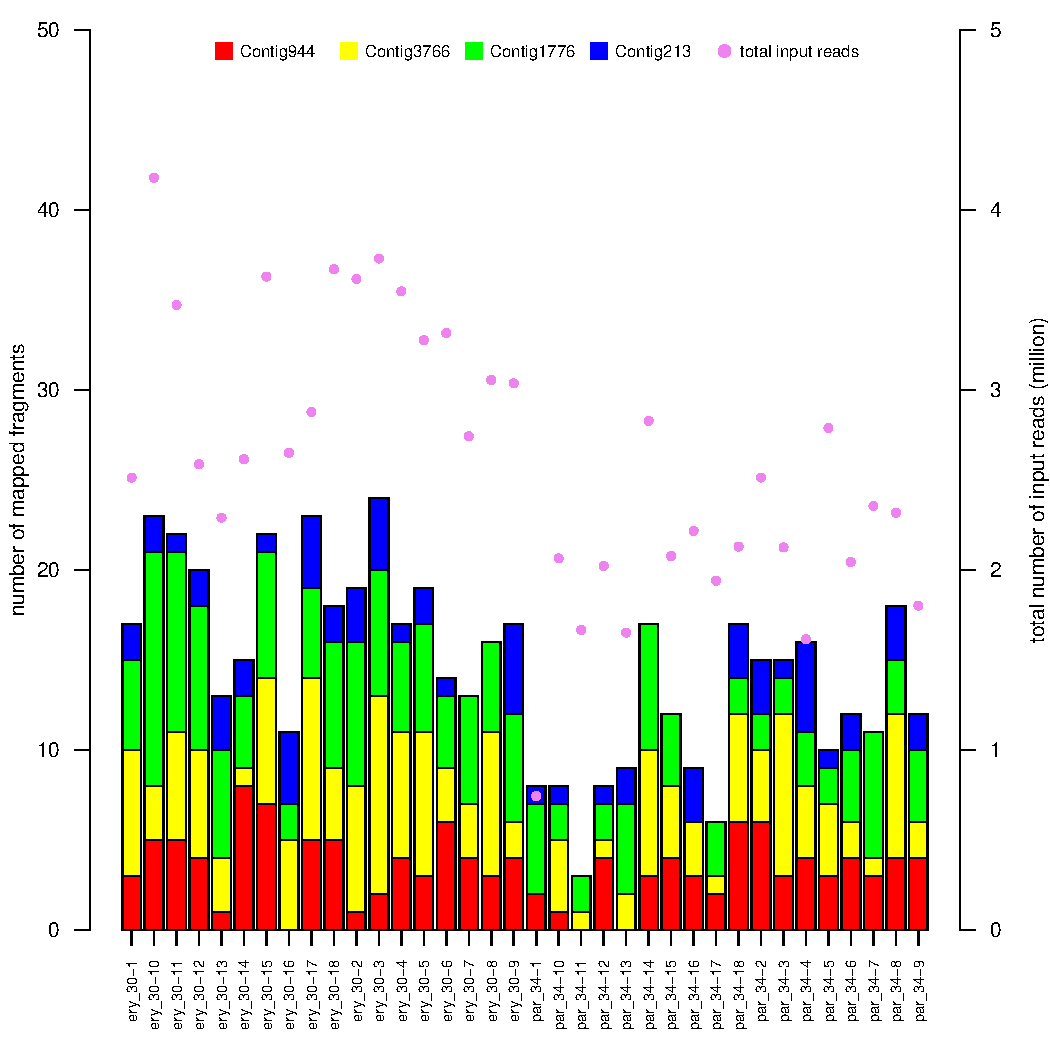
\includegraphics[width=.9\linewidth]{figure/fragments_mapped_per_ind-1} 

}



\end{knitrout}
\caption{Distribution of RAD \gls{fragment} numbers from the 36 individuals in the library mapped against 4 \emph{PE contig pair} reference sequences.}
\label{fragments-mapped-per-ind}
\end{figure}
%

I combined pairs of PE contigs by aligning them to their putative \textit{Schistocerca} reference contig and filled the gap between them with N's. I then used these 20 newly created \textit{C. parallelus} consensus sequences as a reference against which to map all standard SbfI RAD reads (further details in section \ref{ch:Backmapping}). That is because before setting out to do PCR I wanted to find out how many of the 36 individuals get reads mapped to these \glspl{linked RAD tag site} and whether individuals actually have reads mapped to both \glspl{RAD tag} at an SbfI restriction site. This could be important information for prioritising some of the 20 loci over others for the analysis of between individual variation in the completeness of digestion with PCR.

Among the 20 \textit{C. parallelus} PE contig pair reference sequences, there are 5 which:

\begin{itemize}
\item do not show very high or very low number of reads mapped
\item do not show large numbers of very divergent reads mostly containing \glspl{indel}
\item do not show other signs of repetitiveness, e. g. SE reads mapping to PE contigs instead of the \glspl{RAD tag}
\end{itemize}

One of these 5 reference sequences has only reads mapped from \textit{C. p. parallelus} (12 individuals) and none from \textit{C. p. erythropus}. This could be caused by a polymorphism in the restriction site sequence. For each individual, I counted the number of \glspl{fragment} mapped towards the remaining four reference sequences by counting only SE reads from \glspl{proper pair} and after removing PCR duplicates by collapsing multiple occurrences of the same insert size into one. If two read pairs on a RAD site from an individual have the same insert size, they constitute only one fragment, i. e. one read pair is likely to be a PCR duplicate. 


Figure \ref{fragments-mapped-per-ind} shows the distribution of these counts over all 36 individuals for the four PE contig pair reference sequences. It suggests that none of the 4 loci would be a good candidate to test possible variation in restriction enzyme digestion with PCR. That is because the distribution of coverage at the 4 loci is rather even across the 36 individuals. Even though between individual variation in the completeness of digestion cannot be ruled out by this data yet, a different pattern would be expected if it was common. That is, more individuals would have no fragments mapping while others would have many. Given this data, a systematic variation in the completeness of restriction enzyme digestion between individuals is now less likely to be the reason for the dominance of singleton loci in the \texttt{stacks} assembly (see figure \ref{freq_dist_of_genotype_calls}). Instead, the variation in coverage among individuals in figure \ref{fragments-mapped-per-ind} can be largely explained by variation in the number of input reads (figure \ref{frag_input_corr_fig}).\todo{add pipeline diagram, use tikz package}
%
\begin{figure}
\begin{knitrout}
\definecolor{shadecolor}{rgb}{0.969, 0.969, 0.969}\color{fgcolor}

{\centering \includegraphics[width=.49\linewidth]{figure/fragments_input_reads_corr-1} 
\includegraphics[width=.49\linewidth]{figure/fragments_input_reads_corr-2} 

}



\end{knitrout}
\caption{Correlation of locus dropout (left) and fragment counts (right) with number of input reads. Left: Locus dropout is the number of loci (which are the same as in figure \ref{fragments-mapped-per-ind}) for which an individual had no \gls{fragment} mapped. Right: the sum of mapped \glspl{fragment} over the four loci for each individual versus the number of input reads for the read mapping.}
\label{frag_input_corr_fig}
\end{figure}

The \gls{fragment} count for the four loci is generally not very high (see table \ref{mean_sd_fragNum_per_locus}), indicating that low unique template amount for sequencing prevented any individual from having many fragments mapped. I started the standard SbfI RAD library preparation with about 130 ng of DNA from each grasshopper. Assuming that the genome is 12 Gbp long (see section \ref{ch:Genome_size}), this would only correspond to around 10,000 copies of the genome (equation \ref{eq:genome_copies}).

%% ---- this is a table, the LaTeX code for which is produced in the accompanying R file: ref-map-doc.R
% latex table generated in R 3.1.2 by xtable 1.7-4 package
% Mon May 11 14:07:54 2015
\begin{table}[ht]
\centering
\caption{Mean and coefficient of variation of fragment counts per individual for the 4 loci shown in figure \ref{fragments-mapped-per-ind}.} 
\label{mean_sd_fragNum_per_locus}
\begin{tabular}{lrr}
  \toprule
 & mean & CV \\ 
  \midrule
Contig944 & 3.5 & 0.5 \\ 
  Contig3766 & 4.5 & 0.6 \\ 
  Contig1776 & 4.8 & 0.5 \\ 
  Contig213 & 1.9 & 0.8 \\ 
   \bottomrule
\end{tabular}
\end{table}

%
For the SbfI$+$XhoI double-digest RAD library I estimated the template amount that went into the selective PCR during library preparation with \textit{q}PCR. This also indicated a very low template amount of on average 1.26 ($\pm$ 0.37) template molecules per locus and individual (see section \ref{ch:qPCR}).
%
\footnotesize
\begin{align}
\text{molar amount of template} &= \frac{\text{amount of DNA}}{\text{MW of bp} \times \text{genome size}} 
= \frac{130 \times 10^{-9}\text{g}}{660 \frac{\text{g}}{\text{mol} \times \text{bp}} \times 12 \times 10^{9} \text{bp}} \label{eq:genome_copies} \\
&= 1.26 \times 10^{-20} \text{mol} \nonumber \\[5pt]
%\end{align}
%\begin{align}
\text{number of template molecules} &= 1.26 \times 10^{-20} \text{mol} \times \text{Avogadro's number} \nonumber \\
&= 1.26 \times 10^{-20} \text{mol} \times 6.0221413 \times 10^{23} \nonumber \\
&= 9884 \nonumber
\end{align}
\normalsize

The problem of low \gls{fragment} count is unlikely to be alleviated much by creating more sequence reads from the same RAD library (figure \ref{PCRduplicates}). Instead, the template amount from each individual for the selective PCR during the library preparation needs to be increased. One obvious way would be to increase the total DNA input from each individual, but that reduces the number of individuals that can be pooled during the library preparation since the capacity of spin columns and the agarose gel (for size selection) is then reached with fewer individuals. Another option could be to postpone the gel fragment size selection until after a selective PCR, thus reducing the loss of template amount before the PCR (see \citealt{Parchman2012} and the table on page \pageref{compProt})\todo{write a new protocol that allows taking 5 to 10 times as much starting DNA as used in previous protocols}.
%
\begin{figure}
\centering
\includegraphics[width=\textwidth]{PCR_duplicates}
\caption{The standard SbfI RAD library was sequenced on four different Illumina GAIIx flow cell lanes with increased sequence template amount resulting in an increased read yield. However, this increased sequencing effort for the same RAD library generated an ever higher proportion of PCR duplicates.}
\label{PCRduplicates}
\end{figure}

If the dominance of singleton loci in the \texttt{stacks} assembly was not caused by a systematic variation in the completeness of digestion between individuals but simply by random dropout due to low template amount, could this in turn again be caused by incomplete restriction enzyme digestion of genomic DNA as indicated by the full \gls{SbfI} recognition sequences found in the RAD sequence data (figure \ref{SbfI_frequency_dist_per_ind})? Or can genomic religation of restriction fragments\footnote{instead of ligation to Illumina adapters} account for the observed restriction enzyme recognition sequences in the \gls{rad} data? \comment{Should I explain here already why it is important the investigate this question? I. e. incomplete digestion much worse than genomic religation.} The rest of this chapter will be investigating this question.


%% --------------------------------------------------
\FloatBarrier
\subsection{Incomplete digestion or genomic religation in the standard RAD library?}
%% --------------------------------------------------

%%% --------------------------------------------------
\subsubsection{Cluster analysis}
%%% --------------------------------------------------

If non-homologous SbfI fragments were ligated during the adapter ligation step in the library preparation, then the subsequences right of the SbfI site in the SE reads should be very divergent within clusters of similar reads, except when the clusters contain PCR duplicates which can be recognised by (almost) identical PE reads\footnote{they should only differ by sequencing errors}. I have therefore collected all read pairs containing an SbfI site from each individual and, after collapsing all identical read pairs into one, clustered these reads by the subsequence left (5') of the SbfI site, thus ignoring the potentially non-homologous subsequence right of the SbfI site (for details see section \ref{cluster_analysis}). Figure \ref{stRAD_all_uniq_SbfI_reads_clustered_1} shows a snapshot from the output.  Even though there clearly is some indication of incomplete digestion (see figure \ref{stRAD_all_uniq_SbfI_reads_clustered_2}), most clusters are largely consistent with genomic religation.
%
\begin{figure}
\centering
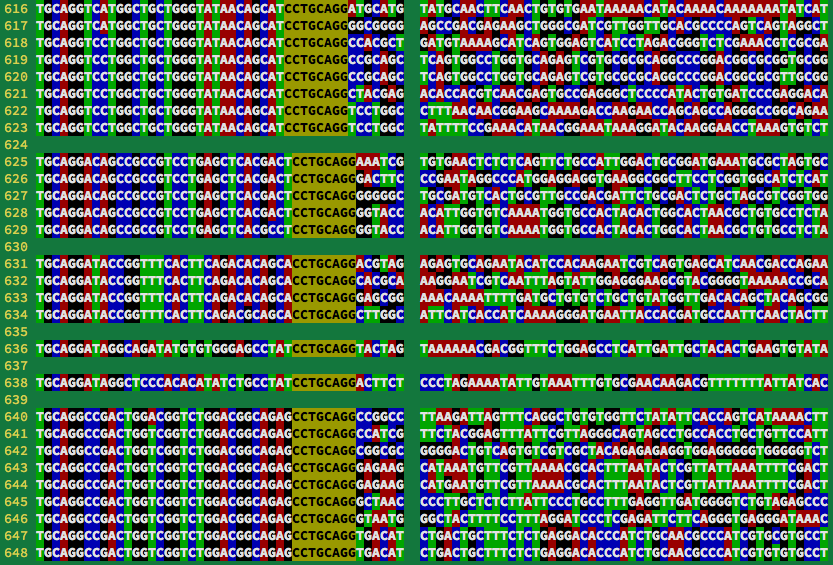
\includegraphics[width=.95\textwidth]{stRAD_all_uniq_SbfI_reads_clustered_1}
\caption{Snapshot of clusters of unique read pairs from the output of command \ref{cmd:cluster_SbfI_reads}. Each line shows a read pair. Left column: SE reads, right column: PE reads. The SbfI recognition sequence is highlighted in yellow. The SE reads in the top cluster are quite diverse right of the SbfI site, although in the lines 619 and 620 as well as 622 and 623 they are identical. In the first case this is clearly due to PCR duplication indicated by the almost identical PE reads (they only differ by sequencing errors). In the second case, however, PCR duplication can be ruled out and only incomplete digestion of the SbfI site at this putative locus seems plausible.}
\label{stRAD_all_uniq_SbfI_reads_clustered_1}
\end{figure}
%
\begin{figure}
\centering
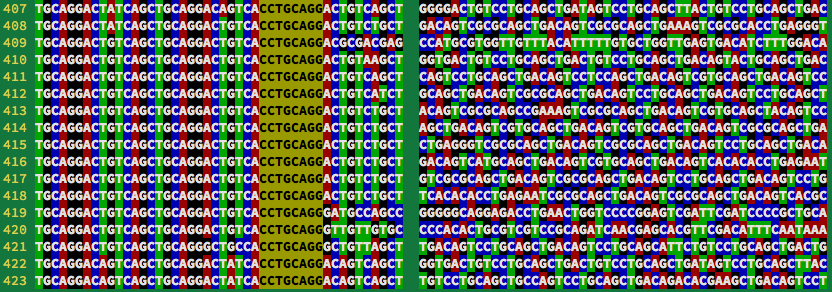
\includegraphics[width=.95\textwidth]{stRAD_all_uniq_SbfI_reads_clustered_2}
\caption{Snapshot of a cluster of unique read pairs from the output of command \ref{cmd:cluster_SbfI_reads}. Each line shows a read pair. Left column: SE reads, right column: PE reads. The SbfI recognition sequence is highlighted in yellow. The sequences right of the SbfI site are not very diverse. In fact, they are so similar that they could be derived from a repetitive genomic element. The read pairs in the lines 413--418, in particular, seem to suggest incomplete digestion of the SbfI site.}
\label{stRAD_all_uniq_SbfI_reads_clustered_2}
\end{figure}

%%% --------------------------------------------------
\FloatBarrier
\subsubsection{Read pair mapping analysis}
%%% --------------------------------------------------

Random genomic restriction fragment religation should create chimeras. If mapped to a reference sequence, read pairs from such chimeras should generally not map as \gls{proper pair}. I therefore mapped all SbfI containing read pairs against the \textit{Locusta migratoria} genome \citep{Wang2014} with \href{http://bowtie-bio.sourceforge.net/bowtie2/index.shtml}{\texttt{bowtie2}} \citep{Langmead2012}. Proper pairs should be a clear indication of incomplete digestion whereas \gls{discordant}ly mapped read pairs could be the result of genomic religation or lack of synteny between the \textit{Chorthippus} and \textit{Locusta} genome or simply the small size of the contigs in the \textit{Locusta} genome assembly.
%%Using command line \ref{cmd:screen_discordant_read_pairs} and my script \texttt{screen.pl}, I counted the number of \gls{discordant}ly mapping read pairs where there is enough space for a properly mapping read pair\footnote{within the limits of 900 bp fragment length that I specified for a proper pair when running \texttt{bowtie2}} on one or the other reference contig.
%
%There are 311 \gls{discordant}ly mapped read pairs where the reads are mapping to (almost) the same mapping position\footnote{with an "=" in column 7 of the SAM record}. These read pairs sometimes clearly overlap each other for a large part (checked with \texttt{Needleman\_Wunsch.pl}). What is odd is that the reported fragment length in column 9 is often even bigger than the read length. Clearly, I don't want to count these reads as \gls{discordant}ly mapped. Instead, I think at least one of each pair should be regarded as unmapped. Since all reportedly discordant read pairs that reportedly map to the same reference contig reportedly map to (almost) the same position, I am discarding SAM records where an "=" sign occurs in the 7th column. Clearly, these are not discordant read pairs that map to distant parts of the same reference contig, which I would have counted as a sign of genomic religation. 
%%
%\begin{cmd}
%\captionsetup{type=cmd}
%\begin{Verbatim}[fontsize=\scriptsize, formatcom=\color{darkgray}, commandchars=\\\{\}]
%
%samtools view -\textcolor{red}{h} -f64 -F14 all_mapped_read_pairs.bam  | awk '$7 !~ "="' | ./screen.pl | wc -l
%\end{Verbatim}
%\caption{\small This command first extracts from read mapping output file in BAM format (binary \gls{SAM}) all SE reads from read pairs where both reads got mapped, but as \gls{discordant} pairs. It then removes lines where the PE read got mapped to the same contig followed by a screen for enough space for a \gls{proper pair} on either reference contig. The remaining  lines are then counted. Note that \texttt{screen.p} needs a \gls{SAM} header to work (red switch).}
%\label{cmd:screen_discordant_read_pairs}
%\end{cmd}
%
%This results in 1525 discordantly mapped read pairs (indicating genomic religation) versus 338 concordant read pairs (indicating incomplete digestion). The average reported mapping quality scores for the two groups of read pairs are quite similar: about 10 for the reads in the proper pair group and about 12 in the reads in the discordant pair group.
%
%In addition to genomic religation, discordant read pairs can be caused by lack of synteny between \textit{Chorthippus} and \textit{Locusta} genome or errors in the \textit{Locusta} genome assembly. 

I therefore tried to estimate the proportion of \gls{concordant}ly mapping read pairs from a random sample of read pairs where, for the vast majority of read pairs, the two reads in a pair should come from the same genomic location as in the case of incomplete digestion. Any reduction in the proportion of \gls{concordant}ly mapping read pairs among the SbfI site containing read pairs with respect to this expectation should be caused by random genomic religation of SbfI restriction fragments. 
%
\begin{figure}
\begin{knitrout}
\definecolor{shadecolor}{rgb}{0.969, 0.969, 0.969}\color{fgcolor}

{\centering \includegraphics[width=.9\textwidth]{figure/read_pair_mapping_analysis-1} 

}



\end{knitrout}
\caption{Density plot from 10,000 samples from the posterior credibility distribution of the differences in $\theta$ between randomly selected reads and SbfI site containing reads. $\theta$ stands for the probability of a read pair to map concordantly.}
\label{fig:read_pair_mapping_analysis}
\end{figure}
%

As a quasi random sample, I have taken the 200,001st to 300,000th read pair from each individual.
After mapping against the \textit{Locusta} genome reference sequences, I first extracted all read pairs where both reads mapped, \gls{concordant}ly or not and disregarding mapping quality. The total number of these read pairs is 846,583. Among these read pairs there are 440,015 that map \gls{concordant}ly (further details from page \pageref{read_pair_mapping_analysis} onwards). So 52\% of mapping read pairs mapped concordantly\todo{That's not that bad. Could I maybe use the \textit{Locusta migratoria} genome as a reference to map all my reads?}. That means that a random read pair -- where both reads generally come from the same genomic location in \textit{C. parallelus} as with incomplete digestion -- is about as likely to map \gls{discordant}ly as \gls{concordant}ly against the \textit{Locusta} genome reference.

Using the same command lines as above for read pairs containing SbfI sites, I counted among a total of 2,184 mapping read pairs 333 which mapped concordantly, or 15.5\%. 

Figure \ref{fig:read_pair_mapping_analysis} shows the posterior credibility distribution of the difference in $\theta$ -- the probability that a read maps concordantly -- between the randomly selected read pairs and the SbfI site containing read pairs. The difference in the probability to map concordantly between a randomly selected read pair and a read pair containing an SbfI site is 0.367 (95\% HDI: 0.352, 0.382). This is a strong difference that says that 37\% \emph{more} reads map concordantly among the randomly selected read pairs than among the SbfI site containing read pairs.

This result is consistent with random genomic religation, which recreates SbfI sites and disrupts concordant mapping of read pairs. If the SbfI sites observed in some reads would only be caused by incomplete digestion, this large difference would not be expected. On the other hand, the fact that 15\% of SbfI site containing reads do map concordantly indicates that genomic religation cannot account for all the observed SbfI sites in the reads.\todo[nolist]{other factors like genomic repetitive sequences or PCR duplicates may have contributed to this deviation.}


%% --------------------------------------------------
\subsection{Incomplete digestion or genomic religation in the double--digest RAD library}
%% --------------------------------------------------

There are also reads from the SbfI$+$XhoI double-digest library that contain full restriction enzyme recognition sequences. I have counted the SbfI and XhoI site positions in \texttt{uniq}-ued \todo{rephrase this} ~\gls{se} and \gls{pe} reads from each individual. The figures \ref{ddRAD_SbfI_frequency_dist} and \ref{ddRAD_XhoI_frequency_dist} show the relative site frequency distributions across SE and PE reads for SbfI and XhoI, respectively (further details in section \ref{site_frequency_distributions}). 
%
\begin{figure}
\begin{knitrout}
\definecolor{shadecolor}{rgb}{0.969, 0.969, 0.969}\color{fgcolor}

{\centering \includegraphics[width=\linewidth]{figure/ddRAD_SbfI_frequency_dist-1} 

}



\end{knitrout}
\caption{Relative SbfI site frequency distributions for the SbfI-XhoI double-digest RAD data set with per individual uniqued reads relative to individual read count. Note that the graph for the PE reads has a 20 times larger y-axis than the graph for SE reads. SE reads are 96 base pairs long, PE reads are 100 base pairs long.}
\label{ddRAD_SbfI_frequency_dist}
\end{figure}
%
%
\begin{figure}
\begin{knitrout}
\definecolor{shadecolor}{rgb}{0.969, 0.969, 0.969}\color{fgcolor}

{\centering \includegraphics[width=.9\linewidth]{figure/ddRAD_XhoI_frequency_dist-1} 

}



\end{knitrout}
\caption{Relative XhoI site frequency distributions for all 38 individuals (including two technical replicates) with per individual uniqued reads relative to individual read count.}
\label{ddRAD_XhoI_frequency_dist}
\end{figure}
%

%%% --------------------------------------------------
\subsubsection{Cluster Analysis}
%%% -------------------------------------------------- 

As with the SbfI site containing reads from the standard SbfI RAD library, if random genomic religation were responsible for the the SbfI and XhoI sites in the double-digest RAD reads, then the subsequences left and right of the SbfI or XhoI sites in the reads should come from different loci. When clustering reads by similarity of the subsequences left of the SbfI or XhoI sites, the subsequences right of the SbfI or XhoI sites should be very divers within clusters.

After collapsing identical SbfI and XhoI site containing SE reads into one, I have therefore clustered them by the subsequence left (5') of the recognition sequence (further details on page \pageref{cluster_analysis}).
Looking into these clusters of uniqued SE reads with XhoI sites does for the vast majority show clusters that are consistent with incomplete digestion (see fig \ref{all_ind_XhoI_in_SE_cl_by_pos})!
%
\begin{figure}
\centering
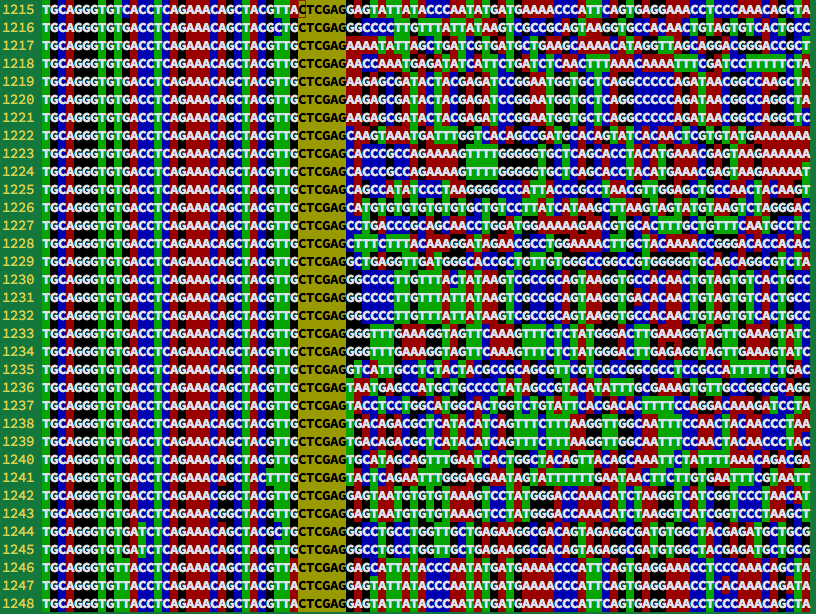
\includegraphics[width=.9\textwidth]{all_ind_XhoI_in_SE_cl_by_pos_1}\\
\vspace{10pt}
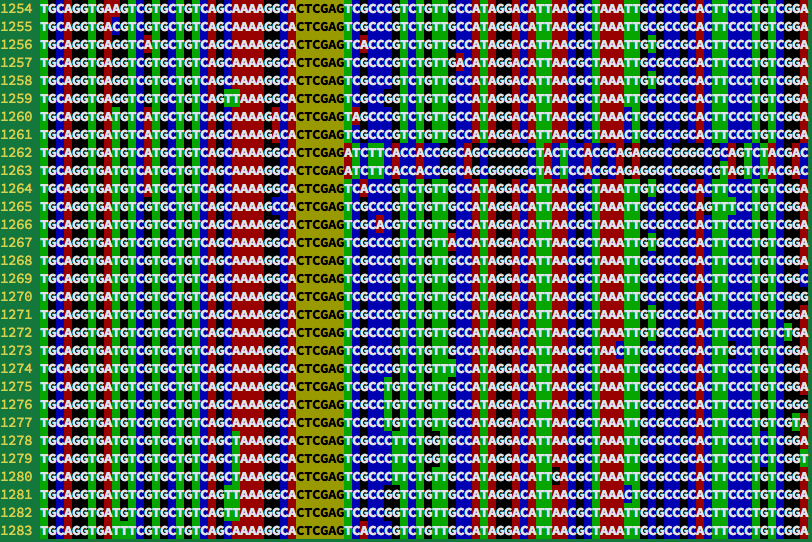
\includegraphics[width=.9\textwidth]{all_ind_XhoI_in_SE_cl_by_pos_2}
\caption{Two clusters produced by \texttt{cluster.pl} on all uniqued SE reads containing an XhoI site. The top cluster is one of only very few that is indicative of genomic religation given its sequence diversity downstream of the XhoI site. The bottom cluster is one of the vast majority (including the many small ones) that are only consistent with incomplete digestion given the lack  of sequence divergence downstream of the XhoI site.}
\label{all_ind_XhoI_in_SE_cl_by_pos}
\end{figure}
%
The clusters from SE reads with an SbfI site, on the other hand, for the vast majority support genomic religation (see figure \ref{all_ind_SbfI_in_SE_cl_by_pos_1}). %
\begin{figure}
\centering
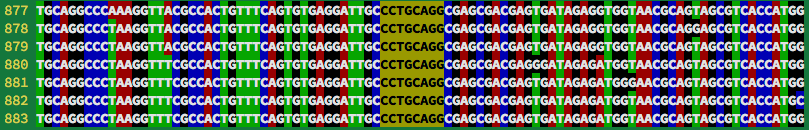
\includegraphics[width=.9\textwidth]{all_ind_SbfI_in_SE_cl_by_pos_1}\\
\vspace{10pt}
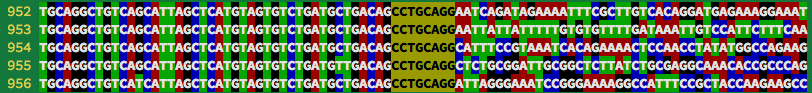
\includegraphics[width=.9\textwidth]{all_ind_SbfI_in_SE_cl_by_pos_2}
\caption{Two examples of clusters produced by \texttt{cluster.pl} on all uniqued SE reads containing an SbfI site. The upper cluster is indicative of incomplete digestion. The lower cluster is indicative of genomic religation.}
\label{all_ind_SbfI_in_SE_cl_by_pos_1}
\end{figure}

%%% --------------------------------------------------------
\subsubsection{Read pair mapping analysis}
%%% --------------------------------------------------------


As for the standard RAD library, if the SbfI or XhoI sites in the reads of the double-digest RAD library are due to random restriction fragment religation, then they should be chimeras. The sequences left and right of the restriction site should map to different parts of a set of genome reference sequences.
That's why I wrote a script called \texttt{digidig.pl} that takes a FASTQ SE read file, looks whether there are SbfI (or XhoI) sites in the reads at a position that leaves at least 30 bp to the left and right of the recognition sequence, splits the reads at the SbfI (or XhoI) site and writes the upstream part to a new SE file and the reverse complement of the downstream part to a new PE file. Next, I mapped these individual paired read files against the \textit{Locusta} reference genome \citep{Wang2014} with \texttt{bowtie2}. I have then extracted all reads from read pairs where both reads mapped, properly or not and disregarding mapping quality (see page \pageref{read_pair_mapping_analysis}).

Using the same command lines as above for the standard RAD read pairs, but specifying an accepted insert size range of 30 till 120 (instead of 50 till 900), I counted 116 \gls{concordant}ly mapped read pairs (indicating incomplete digestion) among a total of 932 mapped read pairs (12.4\%).

I have also digitally digested the SE reads with XhoI using \texttt{digidig.pl} and mapped the digested reads against the \textit{Locusta} genome reference. Using the same methods as for SbfI site containing SE reads, I counted 949 read pairs mapping concordantly (indicating incomplete digestion) among a total of 2250 mapped read pairs (42.2\%).

%But what is the expected proportion of \gls{discordant}ly versus concordantly mapped read pairs from reads that do not contain SbfI or XhoI recognition sequences, i. e. reads that cannot be derived from genomic religation?
%
%I assume that if I had digitally digested random read pairs from the SbfI-XhoI ddRAD data set, I would have gotten a similar ratio of properly versus discordantly mapped read pairs. So finding among the SbfI-digitally digested ddRAD SE reads more than 10 times more mapping as discordant read pairs than proper read pairs should also be a significant deviation indicating that most SbfI sites in these reads are caused by genomic religation.
%
%The XhoI-digitally digested ddRAD SE reads, on the other hand, only slightly deviate from the roughly 1:1 ratio of proper versus discordant read pairs indicating that most XhoI sites in SE ddRAD reads are caused by incomplete digestion.

In order to estimate the expected proportion of \gls{concordant}ly mapping read pairs for reads where both read subsequences are derived from the same location in the \textit{C. parallelus} genome (as with incomplete digestion), I modified \texttt{digidig.pl} to also allow \emph{random digital digestion}. It picks a random cut position while making sure that each new read in the resulting read pair is at least 30 bp long. 

As a quasi random sample of reads I took the 200,001st -- 300,000th SE reads \todo{mention that these reads were base call quality cleaned and trueTags filtered?} from each individual. I then digitally digested these random reads randomly with \texttt{digidig.pl} creating new read pairs with variable read lengths. I then mapped these read pairs against the \textit{Locusta} genome reference with \texttt{bowtie2} with the same settings as before (see page \pageref{read_pair_mapping_analysis})\todo{check wether internal references are correct}. I used the same set of command lines as above for the SbfI and XhoI digitally digested SE reads. I thus counted 689,319 \gls{concordant}ly mapping read pairs among a total of 1,041,305 mapping read pairs, or 66.2\%.

%% ---------------------------------------------
\subsection{Summary}
%% ---------------------------------------------

Table \ref{tab:mapping_summary} summarises the mapping results for the two different RAD libraries and the two restriction enzymes used and shows that reads with SbfI sites map concordantly much less often than would be expected if they were mainly caused by incomplete digestion. Reads containing XhoI sites, on the other hand, map concordantly much more frequently, although still far fewer than expected if incomplete digestion were the sole reason for XhoI sites in these reads.
%
\begin{table}
\centering
\caption{\small Summary of results from read pair mapping analyses. The percentage of concordantly mapping read pairs is shown for each data set together with the expected percentage from random read pairs.}
\label{tab:mapping_summary}
\vspace{5pt}
\begin{tabular}{lcc}
\toprule
\multirow{2}{*}{data} & \multicolumn{2}{c}{\% concordant} \\
                                    & observed & expected \\
\midrule
SbfI in standard RAD & 15.5 & 52.0  \\
SbfI in ddRAD & 12.4 & 66.2 \\
XhoI in ddRAD & 42.2 & 66.2 \\
\bottomrule
\end{tabular}
\end{table}
%
These results are consistent with the results from the analysis of clusters of cut site containing reads. 

So incomplete digestion seems to have affected XhoI sites much more than SbfI sites in both types of RAD libraries. 
In order to detect an XhoI site that was not cut within SE reads of the double-digest library, it (i) needs to be within less than 90 base pairs of the SbfI site and (ii) have a second XhoI site within the next few hundred base pairs that \emph{was} cut, so that a P2 adapter could be ligated. Given these highly restrictive conditions, it seems likely that incomplete digestion of XhoI sites has significantly reduced the template amount for the SbfI$+$XhoI double-digest RAD library.

Incomplete digestion is a much more severe problem with the library preparation than genomic religation. When assembling \glspl{RAD tag} only from SE reads as in standard RAD, genomic religation should only interfere with clustering when the second restriction site is within a read length of the first. Other chimeras should not be a problem for clustering. By contrast, incomplete digestion does not so much interfere with \gls{RAD tag} assembly -- two SbfI sites within a read length of each other should be rare anyway -- but it indicates that an unknown (and probably unknowable) fraction of restriction sites were not cut. That is because an uncut site can only be detected if there was a restriction site close by that \emph{did} get cut. So, the indication that the SbfI restriction sites in the reads of the two RAD libraries are probably mostly due to genomic religation is a good sign, although it indicates an inefficient ligation of Illumina adapters, which also reduces PCR template amount. The general lack of signs for genomic religation in the SE reads containing an XhoI site, on the other hand, is reason for concern, since it suggests incomplete digestion. \todo{mention methylation sensitivity}

Given the rarity of signs for incomplete digestion of SbfI restriction sites, it seems unlikely that it alone could have reduced the template amount enough to cause the extreme skew in the distribution of putative \gls{RAD tag} loci over genotype calls (i. e. individuals) as observed in figure \ref{Big_Data:freq_dist_of_genotype_calls}.

%\section{Discussion}
%
%\begin{itemize}
%\item \todo[inline,nolist]{read \cite{Ilut2014}}
%\item \todo[inline,nolist]{explain challenge of large repetitive genome}
%\item \todo[inline,nolist]{most analyses just take the called loci unquestioned, assumption that this is an unbiased sample of loci, provide examples}
%\item \todo[inline,nolist]{what about repeatability, if only a few 1000 of $>$100,000 loci are studied}
%\item \todo[inline,nolist]{this data is just an example of problems that can occur with RAD}
%\item \todo[inline,nolist]{mention that template amount dependent on the genome size}
%\item \todo[inline,nolist]{mention methylation as possible reason for incomplete digestion}
%\item \todo[inline,nolist]{recommendations for future studies}
%\item \todo[inline,nolist]{write new ddRAD protocol incorporating the Parchman and Peterson protocols}
%\end{itemize}

%\begin{comment}
%\end{comment}

%% ---------------------------------------------------
%\clearpage
\section{Methods}
%% ---------------------------------------------------

All commands and programmes shown here have been executed in the command processor \href{http://en.wikipedia.org/wiki/Bash_%28Unix_shell%29}{BASH} on the  Debian-based Linux operating system called \href{http://en.wikipedia.org/wiki/Ubuntu_%28operating_system%29}{Ubuntu}.

%% ---------------------------------------------------
\subsection{Adapter sequences for SbfI$+$XhoI ddRAD}\label{ch:adapter_sequences}
%% ---------------------------------------------------

%\begin{minipage}[c][5cm][c]{1.2\textwidth}
\begin{figure}[H]
%, frame=single, framesep=10pt, label=P1 and P2 adapters for ddRAD]
\begin{Verbatim}[fontfamily=courier, fontsize=\relsize{-7}, commandchars=\\\{\}] 
          {\footnotesize P1 adapter}                                        {\footnotesize insert}                                   {\footnotesize P2 adapter}
5'-\underline{AATGATACGGCGACCACCGA}GATCTACACTCTTTCCCTACACGA\colorbox{white}{CGCTCTTCCGATCT}xxxxx{\color{blue}TGC*A}     GGNNNNNNNNNNNC     P-{\color{red}TCGA}\colorbox{orange}{A-GATCGGAAGAGCG}GTTCAGCAGGAATGCCGAGACCG\rotatebox{30}{\textit{TAGAGCATA*C}-3'}
3'-TTACTATGCCGCTGGTGGCTCTAGATGTGAGAAAGGGATGTGCT\colorbox{orange}{GCGAGAAGGCTAGA}xxxxx-P    {\color{blue}ACGT}CCNNNNNNNNNNNG{\color{red}AGCT}       \colorbox{white}{T*CTAGCCTTCTCGC}CAAGTCGTCCTTACGGCTCTGGCTAG\underline{AGCATACGGCAGAAGACGAAC-5'}
\end{Verbatim}
\caption{Outline of P1 and P2 adapters for double-digest RAD. Underlined sequences are selective PCR primer sequences. An asterisk * stands for a phosphorothioate bond. A "P" stands for a phosphate group. Sequences in \textit{italics} are non-complementary (wavy). Sequences with an orange background are identical to each other. An "x" stands for a base in a barcode sequence.}
\label{adapter_outline} % note, label has to come after caption
\end{figure}
%\end{minipage}


%% ---------------------------------------------------
%\FloatBarrier
\subsection{Estimating genome wide GC content}\label{ch:gc}
%% ---------------------------------------------------


%
\begin{cmd}
\captionsetup{type=cmd} % this is necessary for the hyperlink to work, see manual for caption package, 6.5 about hyperref
\begin{Verbatim}[formatcom=\color{darkgray}, fontsize=\scriptsize]

for i in *fq_2.gz; 
do 
( awk '(NR-2)%4==0' <(zcat $i) | perl -ne' $h{$_}=1;END{foreach $s (keys %h)
{$gc += $s =~ tr/GC/GC/;} print $gc/(51 * scalar keys %h), "\n";} ' )& 
done | \
perl -ne'$sum+=$_; END{print $sum/$., "\n";}'

0.4607
\end{Verbatim}
\caption[Determine GC content from standard RAD PE reads]{\small For each individual, this command takes the \glspl{pe} reads, uniques them and determines their overall GC content. Finally, the average of the individual GC contents is taken. Note the brute-force parallelisation by sending each iteration of the \texttt{for} loop into the background with \texttt{(\ldots )\&}.}
\label{cmd:GC_1}
\end{cmd}
%
Using the \gls{se} reads from the \gls{SbfI} RAD library (excluding the SbfI recognition sequence part) and command \ref{cmd:GC_2} I have determined the GC content of the \gls{se} reads: 49.5\%. So, it seems that sequences close to \gls{SbfI} sites are more GC rich than further distant sequences. 
%
\begin{cmd}
\captionsetup{type=cmd} % this is necessary for the hyperlink to work, see manual for caption package, 6.5 about hyperref
\begin{Verbatim}[formatcom=\color{darkgray}, fontsize=\scriptsize, numbers=left]
gc(){ awk '(NR-2)%4==0' | sed 's/^......//' | \
perl -ne'$h{$_}=1;END{foreach $s (keys %h){$gc+=$s=~tr/GC/GC/;} 
print $gc/(40*scalar keys %h), "\n";}' ;}

export -f gc

mean(){ perl -ne'$sum+=$_; END{print $sum/$., "\n";}'; }

export -f mean

parallel -j 10 'zcat {} | gc' ::: *fq_1.gz | mean

0.4956
\end{Verbatim}
\caption[Determine GC content of \gls{se} reads]{\small This command is a different version of command \ref{cmd:GC_1}. It is used here to determine the GC content of all \gls{se} reads from the standard \gls{SbfI} RAD library. It first creates and exports two functions, \texttt{gc} and \texttt{mean}, and then uses the programme \texttt{parallel} in order to parallelise the determination of GC content over 10 cores. After stripping barcode and the remainder of the restriction site, the reads are 40 base pairs long. Note, the space between \{ and \texttt{awk} (line 1) as well as \{ and \texttt{perl} (line 7) is required.}
\label{cmd:GC_2}
\end{cmd}



%% --------------------------------------------------------------------------------------------------------------------------
\FloatBarrier
\subsection{Genome size of \textit{Chorthippus parallelus}}\label{ch:Genome_size}
%% --------------------------------------------------------------------------------------------------------------------------

\textit{Chorthippus parallelus} has a chromosome complement of 2n = 16 + X. Males have one X-chromosomes, females have two. Table \ref{ta:genome_size_studies} shows four studies that provide genome size estimates for \textit{Chorthippus parallelus}. Note that all studies are measuring the DNA content of spermatids. However, none of the studies explicitly deal with the issue that half of their measurements are missing the contribution from the X chromosome. Table \ref{ta:genome_size_studies} mentions the country of origin of the grasshoppers used for genome size estimates. Note, however, that only \cite{Belda1991} provide sampling locations. For the rest it is assumed that individuals were sampled close to the authors institutes. So two studies provide genome size estimates for \textit{C. parallelus parallelus} and two for \textit{C. parallelus erythropus}. The \textit{parallelus} subspecies seems to have a genome 2--4 giga \glspl{bp} larger than the one of subspecies \textit{erythropus}. Apart from possible systematic differences in methodology, this apparent difference in genome size could be real, since several studies have shown chromosomal differentiation between the two subspecies, in particular on the X chromosome: an active nucleolar organiser region (NOR) distally on the X in \textit{C. p. parallelus} but not in \textit{C. p. erythropus} \citep{Gosalvez1988}. This NOR on X lies in or near a distinctive distal C-band\footnote{\gls{heterochromatin} stained with Giemsa}. In addition, Pyrenean \textit{C. p. erythropus} also show an interstitial C-band on X that does not occur in pure \textit{C. p. parallelus} \citep{Bella2007}. Further chromosomal differences are listed in table 1 of \cite{Ferris1993}.

\ctable[
width=\textwidth,
doinside={ \relsize{-1.5} \setlength{\tabcolsep}{3pt} },
caption=Studies that provide genome size estimates for \textit{Chorthippus parallelus},
cap=Genome size estimates,
label=ta:genome_size_studies
]
{l c >{\raggedleft}p{.6cm}@{.}l >{\centering}p{2.5cm} l X}
{
\tnote[a]{\scriptsize see their table 3}
\tnote[b]{\scriptsize 5 individuals}
\tnote[c]{\scriptsize assuming 6.4 on relative scale corresponds to C-value of 5.5 pg}
\tnote[d]{\scriptsize see their table 2}
\tnote[e]{\scriptsize \textit{C. longicornis} syn. of \textit{C. parallelus}}
\tnote[f]{\scriptsize 3 individuals}
\tnote[g]{\scriptsize 3 individuals}
}
{
\toprule
\multirow{2}{*}{\textbf{study}} & \multirow{2}{1cm}{\textbf{sample source}}  & \multicolumn{2}{c}{\textbf{C-value}} & \multirow{2}{*}{\textbf{Method}} & \multirow{2}{*}{\textbf{tissue type}} & \multirow{2}{*}{\textbf{standard species}} \\
                                      &                                                              & \multicolumn{2}{c}{ [$10^{-12}$g]} &                                &                                                 &                                                           \\
\midrule
\cite{John1966}\tmark[a] & UK & 12&37 ($\pm$ 0.75)\tmark[b] & Feulgen staining, microdensitometry & spermatid & \textit{Locusta migratoria}\tmark[c] \\[0.3cm]
\cite{Wilmore1975}\tmark[d] & UK & 13&36 ($\pm$ 0.04) & Feulgen staining, microdensitometry & spermatid & mouse spermatid \\[0.7cm]
\cite{Gosalvez1980}\tmark[e] & Spain & 8&58 ($\pm$ 0.47)\tmark[f]   & Feulgen staining, microdensitometry & spermatid & \textit{Allium cepa}, root tissue \\[0.3cm]
\cite{Belda1991} & Spain & 10&73 ($\pm$ 0.97)\tmark[g]  & Feulgen staining, microdensitometry & spermatid & chick erythrocytes \\
\bottomrule
}

\cite{Gosalvez1988} showed that all the heterochromatin present in both subspecies is particularly rich in GC DNA base pairs\todo{This would suggest using restriction enzymes for RAD with recognition sequences rich in AT in order to preferentially target transcribed regions of the genome.}.


%\begin{table}
%\caption{Studies that provide genome size estimates for \textit{Chorthippus parallelus}}
%\label{ta:genome_size}
%\centering
%\small
%\resizebox{\textwidth}{!}{
%\begin{tabular}[h]{c c >{\raggedleft}p{.6cm}@{.}l >{\centering}p{3cm} c c}
%\toprule
%\multirow{2}{*}{\textbf{study}} & \multirow{2}{1cm}{\textbf{sample source}}  & \multicolumn{2}{c}{\textbf{C-value}} & \multirow{2}{*}{\textbf{Method}} & \multirow{2}{*}{\textbf{tissue type}} & \multirow{2}{*}{\textbf{standard species}} \\
%                                      &                                                              & \multicolumn{2}{c}{ [$10^{-12}$g]} &                                &                                                 &                                                           \\
%\midrule
%\cite{John1966} & UK & 12&37 $\pm$ 0.75 & Feulgen staining, microdensitometry & spermatid & \textit{Locusta migratoria}\\[0.7cm]
%\cite{Wilmore1975} & UK & 13&36  & Feulgen staining, microdensitometry & spermatid & mouse spermatid \\[0.7cm]
%\cite{Gosalvez1980} & Spain & 8&58   & Feulgen staining, microdensitometry & spermatid & \textit{Allium cepa}, root tissue \\[0.7cm]
%\cite{Belda1991} & Spain & 10&73  & Feulgen staining, microdensitometry & spermatid & chick erythrocytes \\
%\bottomrule
%\end{tabular}
%}
%\end{table}


%% --------------------------------------------------------------------------------------------------------------------------
\FloatBarrier
\subsection{Expected RAD marker number}\label{ch:RAD_marker_number}
%% --------------------------------------------------------------------------------------------------------------------------

Using PE reads from the standard RAD library -- uniqued  per individual -- as a proxy for the whole genome, I estimate the GC content of the \textit{Chorthippus parallelus} genome to be around 46\% (\ref{ch:gc}). However, \cite{Wilmore1975} have determined the GC content of the \textit{C. p. parallelus} genome from thermal dissociation profiles (41.2\%) and sedimentation in CsCl and Cs$_{2}$SO$_{4}$ density gradients (41.7\% and 42.0\%)\footnote{see their table 1}. I think that \gls{pe} reads from SbfI standard RAD are still a biased sample towards GC rich regions of the genome due to the GC rich \gls{SbfI} recognition sequence. 
Assuming a genome size of 12 giga base pairs, the expected number of RAD tag loci from a standard RAD library with \gls{SbfI} in the grasshopper genome is $\sim$170,000 (equation \ref{eq:exp_num_standard_RAD_loci}). 

\scriptsize
\begin{align}
\text{expected number of \glspl{RAD tag}} &= \underbrace{12 \times 10^{9}}_{\text{genome size}} \times 
\underbrace{ \left( \frac{0.42}{2}\right)^{6} \times \left( \frac{(1-0.42)}{2} \right)^{2} }_{\text{SbfI site probability}} \times 
\underbrace{2}_{\text{tags per SbfI site}}
\label{eq:exp_num_standard_RAD_loci} \\[5pt] 
&= 173,110 \nonumber
\end{align}
\normalsize

The number (and identity) of markers in a double-digest RAD library depends very much on the size selection of restriction fragments. I selected fragments roughly between 300 and 800 \gls{bp} length. The P1 adapter is 63 bp long (excluding 4 bp overhang), the P2 adapter is 61 bp long (excluding 4 bp overhang). The \gls{SbfI} remainder after the cut is 6 \gls{bp} long and the \gls{XhoI} remainder is 5 \gls{bp} long. If \gls{XhoI} cuts a fragment at a distance less than about $300 - 63 - 61 -6 -5 = 165$ \gls{bp} away from the SbfI cut site, then this fragment would not be size selected because it would be shorter than the lower bound of size selection (in this example). The \gls{se} sequences (excluding the SbfI recognition sequence parts) have a mean GC content of 49.5\% (see command \ref{cmd:GC_2}). 
The following formula requires the GC content of sequences of length 168 \gls{bp} adjacent to SbfI sites. I will use the average of \gls{se} and \gls{pe} GC contents -- 48\% (see~chapter \ref{ch:gc}) -- for calculating the probability of no XhoI cut within the first 168bp after the SbfI restriction site. In the next 500 \gls{bp} then needs to be at least one \gls{XhoI} site to make the SbfI fragment a marker.
The expected number of RAD markers per genome with an SbfI-XhoI double-digest and a selected size range of 300--800bp is:


\scriptsize
%\begin{preview}
\begin{align} % use align instead of equation for multi-line long equations
\text{RAD markers per genome} &\simeq 12 \times 10^{9} 
	&&\text{(genome size in bp)}  \label{eq:exp_number_ddRAD_loci} \\[5pt]
&\times \left(\frac{0.42}{2}\right)^{6}\times \left(\frac{(1-0.42)}{2}\right)^{2} &&\text{(SbfI cut prob. per bp)} \notag \\[5pt]
&\times 2 
	&&\text{(each cut creates two potential RAD tags)} \notag \\[5pt]
&\times \left[1-\left(\frac{0.48}{2}\right)^{4} \times \left( \frac{(1-0.48)}{2}\right)^{2} \right]^{165} 
	&&\text{(prob. of no XhoI cut in the first 165 bp after SbfI site)} \notag \\[5pt]
&\times \left(1- \left[1-\left(\frac{0.46}{4}\right)^{2} \times \left( \frac{(1-0.46)}{4}\right)^{4} \right]^{500} \right) 
	&&\text{(prob. of at least one XhoI cut in the following 500bp)} \notag \\[5pt]
%&\quad \times \ 2 \tag{two markers per SbfI cut{\color{red}*}}  \\
&\simeq 16,000 \nonumber
\end{align}
%\end{preview}
\normalsize

I have created an Excel file called \texttt{ComplexityReduction.xls} that implements equation \ref{eq:exp_number_ddRAD_loci} and that allows easy modification of variables.

%%% ---------------------------------------------------
%\FloatBarrier
%\subsection{Quality filtering and pre--processing raw data}
%\label{ch:Qfilt}
%%% ---------------------------------------------------
\todo{add section about quality filtering and pre-processing raw data}

%% ---------------------------------------------------
\FloatBarrier
\subsection{Assembling pairs of PE read contigs}\comment{Are we assembling contigs from reads or are we assembling reads into contigs?}
\label{ch:read_mapping}
%% ---------------------------------------------------

\paragraph{Read mapping}
The 49 million standard SbfI RAD reads used here were base call quality filtered with \texttt{process\_radtags}\footnote{from the \texttt{stacks} pipeline} and a quality score threshold of 20 in a 20 bp sliding window. \texttt{process\_radtags} also made sure that the remainder of the SbfI restriction site was present at the 6th position in the SE reads and that it was preceded by one of the 36 5 bp long \glspl{barcode} that I used, for each case allowing 1 bp mismatch. I mapped these reads against the \textit{Schistocerca} transcriptome \citep{Badisco2011} with \texttt{stampy} \citep{Lunter2011} and setting the switches \texttt{--noautosense}, to turn off inference of insert size distribution, and \texttt{--insertsd=400}, to specify a very wide insert size distribution. This is to ensure that the \gls{proper pair}  bit in the \href{http://samtools.github.io/hts-specs/SAMv1.pdf}{SAM flag} is set correctly by \texttt{stampy}. I then used command \ref{cmd:sam_to_bam_via_awk_in_parallel} in order to extract all \gls{SAM} records, where at least one read from a pair got mapped, with subsequent position sorting.
%
\begin{cmd}
\captionsetup{type=cmd} % this is necessary for the hyperlink to work, see manual for caption package, 6.5 about hyperref
\begin{Verbatim}[fontsize=\scriptsize, formatcom=\color{darkgray}]

for i in *sam.gz; \
do (samtools view -hS $i | gawk '/^\@/ || and($2, 4)==0 || and($2, 8)==0' | \
samtools view -uhS - | samtools sort - `basename $i .fq_1.sam.gz`) & done
\end{Verbatim}
\caption{\small Command line that uses \texttt{samtools} and \texttt{awk} to create position sorted bam files in parallel that only contain records of paired reads where at least one read of the pair got mapped (i. e. skipping records with flag 77 and 141). \scriptsize{Note the brackets around the command line and the skipping of ";" between "\&" and "done"}. }
\label{cmd:sam_to_bam_via_awk_in_parallel}
\end{cmd}
%
After this filtering, I merged all individual mapping output files into one big file with \texttt{samtools merge}.
Note, that I did not filter for \glspl{mqs}, so that reads with ambiguous mapping position\footnote{with quality score $<3$, see \texttt{stampy} README section 11.5} were also retained. When \texttt{stampy} identifies several equally good mapping locations for a read or read pair, it reports one of these at random. Also note that the \textit{Schistocerca} \glspl{EST} were assembled with the programme \href{http://www.phrap.org/phredphrap/general.html}{\texttt{phrap}} and the authors do not report any attempt to merge different transcripts from the same gene into so-called unigenes. It can therefore happen that reads that are derived from the same position in the genome map to different parts of the \textit{Schistocerca} reference.\addcit{\cite{Cahais2012}}

%
%
%

\paragraph{Detecting linked rad tag sites}\label{ch:find_linked_RADtags}
The programme \href{http://www.broadinstitute.org/software/igv/home}{\texttt{IGV}} among others can be used to visualise the alignment of many reads against a set of reference sequences. However, visually inspecting all \textit{Schistocerca} reference contigs for whether they have read pairs mapped to both sides of one SbfI restriction site is very tedious and time consuming. That is why I wrote the script called \texttt{find\_linked\_RADtags.pl} which reports reference contigs where at least two read pairs map to opposite sites of an SbfI restriction site (or any cut site leaving a 4 bp overhang). This script also detects the contig shown in figure \ref{LC.1628.C1.Contig1776_standRAD}. With this script the detection of a reference contig requires one \gls{concordant}ly mapped read pair (also called \gls{proper pair}) on both sides of an SbfI restriction site. So SE as well as PE reads need to map on both sides of the restriction site. This is stringent and will obviously miss contigs with genuine SbfI RAD tag sites, but it is necessary to remove many false positive detections. The purpose of the script is not to detect as many contigs as possible, but only to detect several contigs with genuine SbfI RAD tag sites.\roger{Roger is commenting here.}
%
\begin{figure}
\centering
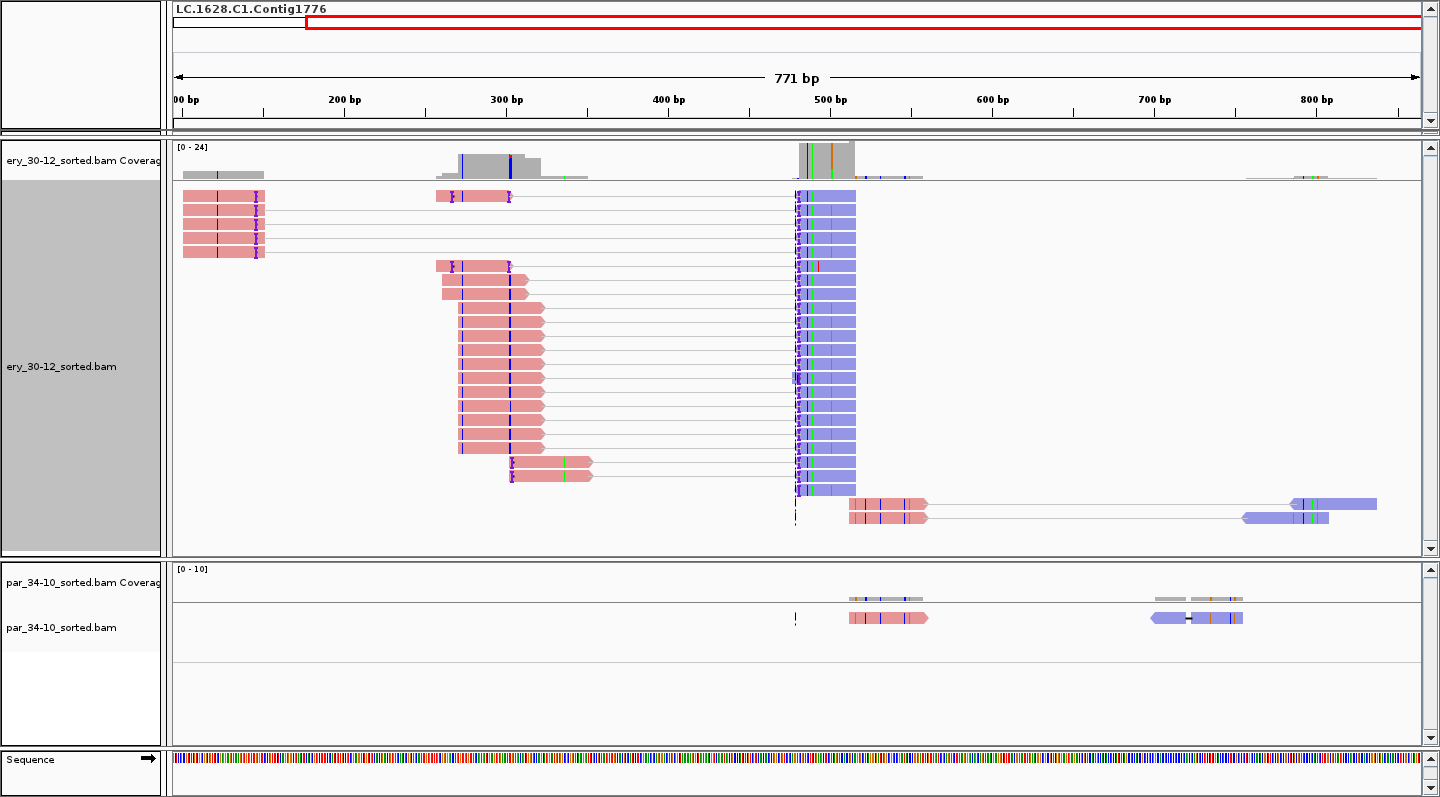
\includegraphics[width=\textwidth]{igv_LC_1628_C1_Contig1776_standRAD}
\caption{Alignment of standard RAD read pairs to both sides of an SbfI restriction site. Read pairs are connected by a line. Forward mapping reads are pink, backward mapping reads are blue. The upper individual has 7 unique read pairs, i. e. with different paired-end reads.}
\label{LC.1628.C1.Contig1776_standRAD}
\end{figure}
%
The script \texttt{find\_linked\_RADtags.pl} collects all \gls{pe} reads that are mates of \gls{se} reads that mapped to a detected \gls{linked RAD tag site}. For each detected reference contig it prints reads upstream or downstream of that site to a separate file. Note, that at this stage \texttt{find\_linked\_RADtags.pl} will only detect one \gls{linked RAD tag site} per reference contig. However, due to the small sizes of the transcriptome contigs, this should not be major shortcoming.

%
%
%

\paragraph{PE read assembly}\label{ch:PE_read_assembly}
I attempted to use \href{http://www.vicbioinformatics.com/software.velvetoptimiser.shtml}{\texttt{VelvetOptimiser.pl}} to assemble the collected \gls{pe} reads into PE contigs \citep{Zerbino2008}. However, the programme fails to assemble three PE read contigs with low read coverage -- Contig1776\_downstream (see figure  \ref{LC.1628.C1.Contig1776_standRAD}), Contig4139\_upstream and LC03019A1F03.f1\_upstream -- despite my diligent attempts to provide the necessary settings \citep{Zerbino2010,Davey2012,Etter2011}.

\texttt{SSAKE} \citep{Warren2007} is a simpler but also less heuristic and more tunable assembly programme than \texttt{Velvet}. It does not take base call quality scores into account and takes only multi-fasta files as input. It searches for \emph{perfect} \gls{kmer} matches between reads. i. e. does not allow for sequencing error or \glspl{snp}.
%
\begin{cmd}
\captionsetup{type=cmd} % this is necessary for the hyperlink to work, see manual for caption package, 6.5 about hyperref
\begin{Verbatim}[fontsize=\scriptsize, formatcom=\color{darkgray}]

for i in ../*fq; do awk '(NR-1)%4==0 || (NR-2)%4==0' $i | \
sed 's/^@/>/' > `basename $i .fq`.fa; done
\end{Verbatim}
\caption[ fastq files into multi-fasta files]{\small Command line that turns fastq files into multi-fasta files. It takes all fastq files in the parent directory, extracts the header and sequence part (while skipping the quality string), replaces the "@" at the beginning of the fastq headers with a required ">" sign and writes the stream to a new file with the same base name.}
\label{fastq_to_fasta}
\end{cmd}
%
\texttt{SSAKE} by default does not allow setting a minimum overlap (\texttt{-m}) of less than 16 \gls{bp}. This could be too stringent for some of the low coverage PE contigs that I wanted to assemble. I, therefore, modified \texttt{SSAKE} to allow a minimum overlap of as small as 10 bp. When calling \texttt{SSAKE} with
%
\begin{description}
\item[\texttt{-w 1}] \textmd{Minimum depth of coverage allowed for contigs}
\item[\texttt{-o 1}] \textmd{Minimum number of reads needed to call a base during an extension}
\end{description}
%
\dots~on the "Contig1776\_downstream" reads from one individual for PE assembly (just two overlapping reads, see fig. \ref{LC.1628.C1.Contig1776_standRAD}), it is able to assemble a full length contig of 81 bp\todo{add comparison of kmer size optimised and un-optimised SSAKE assembly}.

%
%
%

\paragraph{TagCle}
Any non-genomic sequence, i. e. adapter sequence, in the reads should interfere with de novo assembly. The Perl script \texttt{TagCle} by Kang-Wook Kim (Sheffield University) detects overlap between paired reads by Smith-Waterman local alignment and clips off read segments downstream of the end of the local alignment, i. e. generally adapter sequence. That way the script can also detect a \emph{single} adapter (or barcode) base at the end of a read. I used command \ref{tagcle_run} to remove adapter sequences from the reads.
%
\begin{cmd}
\captionsetup{type=cmd} % this is necessary for the hyperlink to work, see manual for caption package, 6.5 about hyperref
\begin{Verbatim}[fontsize=\scriptsize, formatcom=\color{darkgray}]

for i in ../input/*fq_1; 
do 
(j=`echo $i | sed 's/1$/2/'`; TagCle_0.70.pl -me -i1 $i -i2 $j > `basename $i .fq_1`.log) & 
done
\end{Verbatim}
\caption{\small This is the command line that I used in order to run the script \texttt{TagCle} on all 154 pairs of input files in parallel. The \texttt{-me} switch turns off any direct search for adapter sequences.}
\label{tagcle_run}
\end{cmd}
%
\texttt{TagCle} clipped 159 SE and 216 PE reads of a total of 1,584,732 reads (0.02\%). It did not discard any sequence.

%
%
%

\paragraph{Kmer size optimisation}
All de novo assemblers require optimisation of \gls{kmer} length \citep{Davey2012}, which is mainly what \texttt{VelvetOptimiser.pl} does with \texttt{Velvet}. So I wrote a script called \texttt{SSAKEoptimiser.pl} which for each set of PE reads iterates through \gls{kmer} lengths from 11 to 33 and keeps the assembly which produces the longest contig. This script exists in several parallelised versions (using different parallelisation modules) that parallelise not only over input files but also over iterations through \gls{kmer} lengths. This full parallelisation greatly speeds up execution on a multi-core machine (figure \ref{runtimes}).\todo{compare assembly results with and without kmer size optimisation, \texttt{assemblathon\_stats.pl}}
%
\begin{figure}
\centering
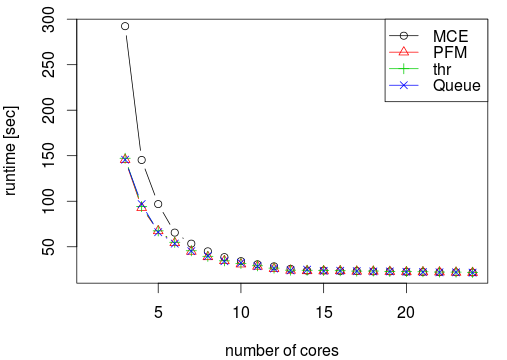
\includegraphics[width=.9\textwidth]{Parallel_Module_Comp}
\caption{The run times of the four parallelised versions of the \texttt{SSAKEoptimiser} script on 11 input files.}
\label{runtimes}
\end{figure}

%
%
%

\paragraph{picking the right \texttt{SSAKE} contigs}\label{ch:picking_right_contig}
\texttt{SSAKE} generally assembles many contigs for a region. In some cases this is due to different SE \glspl{RAD tag} mapping to the same position in the \textit{Schistocerca} transcriptome. In other cases, this is clearly due to insufficient merging of contigs by \texttt{SSAKE} due to low coverage and SNPs (see figure \ref{contig_alignment})
%
\begin{figure}
\centering
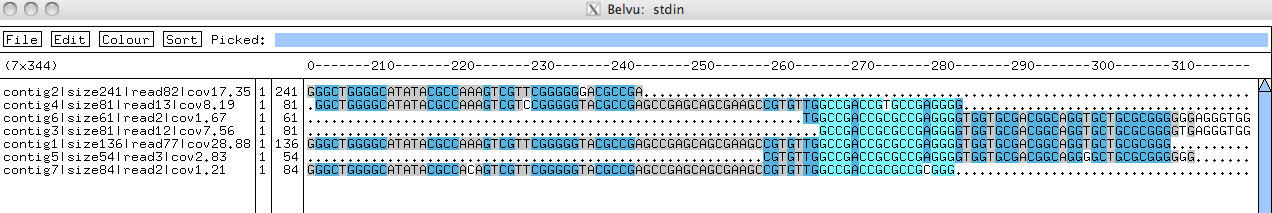
\includegraphics[width=\textwidth]{contig_alignment}
\caption{Multiple sequence alignment of \texttt{SSAKE} contigs assembled from reads collected from the downstream side of the RAD tag site in the \textit{Schistocerca} reference contig "LC.1628.C1.Contig1776". The aligment view was created with the command: \texttt{muscle -in *LC.1628.C1.Contig1776\_downstream*contigs -msf | belvu -}~. The 7 contigs can clearly be merged into one big contig if allowing for a few \glspl{snp}.}
\label{contig_alignment}
\end{figure}
%
That's why I created multiple alignments of \texttt{SSAKE} contigs from each assembly with \texttt{Muscle} \citep{Edgar2004} in order to manually merge them in the alignment editor of \texttt{MEGA} \citep{Tamura2013}.

Since the \texttt{SSAKEoptimiser} output generally contains several \glspl{contig} of similar length and with similar read counts, it is difficult to pick those contigs upstream and downstream that genuinely belong together, i. e. come from the same locus. Visual inspection of a pairwise alignment showed that it is by no means always the longest \gls{contig} assembled that aligns significantly to the \textit{Schistocerca} reference.

In order to help me pick the right \texttt{SSAKE} contigs, I started by determining for each PE read assembly
%
\begin{itemize}
\item the length of the longest contig assembled 
\item the total number of contigs assembled and
\item the number of contigs with length $>100$, $>200$ and $>300$ \gls{bp}
\end{itemize}
%
Another important piece of information would be a significant \texttt{blast} hit of a \texttt{SSAKE} contig against its putative \textit{Schistocerca} reference contig. I therefore extracted all 64 \textit{Schistocerca} reference contig sequences from the \textit{Schistocerca} transcriptome reference file with command \ref{samtools_faidx}.
%
\begin{cmd}
\captionsetup{type=cmd}
\begin{Verbatim}[fontsize=\scriptsize, formatcom=\color{darkgray}]
for i in `cat reference_contig_names_with_up-downstream_contig`; \
do samtools faidx LC_unique.seq  $i > $i.fa; \
done
\end{Verbatim}
\caption{\small Example of a command line that extracts FASTA sequences from an indexed multi-FASTA file using a file listing FASTA headers.}
\label{samtools_faidx}
\end{cmd}
%
With my script \texttt{blast2seq.pl} -- calling \texttt{NCBI blastn 2.2.28+} \citep{Camacho2009} -- I then blasted all 128 relevant \texttt{SSAKE} contig files against their putative \textit{Schistocerca} reference contig sequence and recorded the number of blast hits as well as the fasta headers of the 10 best hitting \texttt{SSAKE} contigs together with their \gls{e-value} (\href{http://blast.ncbi.nlm.nih.gov/Blast.cgi?CMD=Web&PAGE_TYPE=BlastDocs&DOC_TYPE=FAQ#expect}{further explanation}) in a \textsf{.SSAKE\_contig\_stats} file. I only recorded \texttt{blastn} hits with an \gls{e-value} of less than $10^{-10}$. I then used this table as a guide for picking and possibly merging \texttt{SSAKE} contigs in \texttt{MEGA}. I used command lines similar to \ref{blastn} in order to find overlapping \texttt{SSAKE} contigs that haven't been merged yet.
%
\begin{cmd}
\captionsetup{type=cmd}
\begin{Verbatim}[fontsize=\scriptsize, formatcom=\color{darkgray}]

blastn -query *LC03012A1D06.f1_downstream.fa.ssake*.contigs \
-subject *LC03012A1D06.f1_downstream.fa.ssake*.contigs -task blastn \
-evalue 1e-10 -outfmt 6 | awk '$1 != $2' | sort -k3 -nk11 | awk 'NR%2' | less -S
\end{Verbatim}
\caption{\small This command line example is a very quick way to find out which sequences in a multi fasta file are similar to each other. It prints out hits of an all by all \texttt{blastn} of the sequences in a file. Note that query and subject get the same file. The first \texttt{awk} command removes hits against itself, the sort part brings reciprocal hits together and the second \texttt{awk} command keeps only one line for each pair of matching sequences.}
\label{blastn}
\end{cmd}

I only called pairs of PE contigs if on each side of the restriction site I could unambiguously pick a \texttt{SSAKE} contig. This either required a much better blast hit than the second best \texttt{SSAKE} contig or, if no blast hits could be obtained, a small number of \texttt{SSAKE} contigs, one of them being much longer than the others. I required at least one of the two PE contigs from a restriction site to have a significant blast hit to the \textit{Schistocerca} reference contig.

After picking and potentially merging \texttt{SSAKE} contigs, I aligned upstream and reverse complemented downstream contigs against their putative \textit{Schistocerca} reference contig (if possible, i. e. significant blast hit) and filled the gap between them with N's. I thus created a new \textit{C. parallelus} PE contig pair consensus sequence for each \textit{Schistocerca} reference contig. 

%% ---------------------------------------------------------------------------------------------
\FloatBarrier
\subsection{Backmapping}\label{ch:Backmapping}
%% ---------------------------------------------------------------------------------------------

After the creation of 20 \textit{C. parallelus} PE contig pair consensus sequences, I wanted to find out how many of the 36 individuals get reads mapped to these 20 \glspl{linked RAD tag site} and whether individuals actually have reads mapped to both sides of an SbfI restriction site. 

\paragraph{Including se rad tag sequences into the new reference}
Before mapping all standard SbfI RAD reads back against the newly created PE contig pair reference, I wanted to include the SE \gls{RAD tag} sequences into the PE contig pair consensus sequences. For the determination of the consensus \gls{RAD tag} sequences I obviously only want to use reads whose PE mate was used for the assembly of the \texttt{SSAKE} PE contig that I finally picked (see section \ref{ch:picking_right_contig}). That's because the script \texttt{find\_linked\_Radtags.pl} had printed out all read pairs that mapped to a detected \gls{linked RAD tag site} in the \textit{Schistocerca} reference, but after the \texttt{SSAKE} assembly I mostly only picked PE contigs that got a \texttt{blast} hit to their \textit{Schistocerca} reference contig. Other \texttt{SSAKE} contigs are much more likely to derive from similar but non-homologous loci to the \textit{Schistcerca} reference contig. I started by using command \ref{blast_mapping} in order to extract the \href{http://en.wikipedia.org/wiki/FASTQ_format}{FASTQ} headers from those PE reads that get a blast hit to their inferred PE contig.
%
\begin{cmd}
\captionsetup{type=cmd}
\begin{Verbatim}[fontsize=\scriptsize, formatcom=\color{darkgray}]

for i in *fq_2; \
do awk '(NR-2)%4==0 || (NR-1)%4==0' $i | sed 's/@/>/' | sed 's/_pp//' | \
blastn -subject `basename $i .fq_2`_consensus.fas -evalue 1e-10 -outfmt 6 | \
cut -f1 | sed 's/2$/1/' > `basename $i .fq_2`_blast_mapped.ids; \
done
\end{Verbatim}
\caption{\small Using \texttt{blastn} to find PE reads that map to the inferred PE contig (see section \vref{ch:picking_right_contig}). The \texttt{for} loop iterates over all 40 PE read files. The first part of the loop converts fastq to fasta format. The second line feeds that into \texttt{blastn} (using megablast by default) and uses the corresponding PE contig (from section \ref{ch:picking_right_contig}) as subject. The third line takes the first column with the query headers from the blast output table and writes it to an output file.
}
\label{blast_mapping} 
\end{cmd}
%
I then used the output files from this command, containing headers of the required SE sequences, as pattern files for a \texttt{grep} filter of the SE read files that \texttt{find\_linked\_RADtags.pl} has put out (command \ref{grep_filter}).
%
\begin{cmd}
\captionsetup{type=cmd}
\begin{Verbatim}[fontsize=\scriptsize, formatcom=\color{darkgray}]
for i in *ids; \
do grep -A1 -f $i ../all_Big_Data_`basename $i _blast_mapped.ids`.fq_1 | \
egrep -v "\-\-" | sed 's/@/>/' > `basename $i .ids`_SE.fas; \
done
\end{Verbatim}
\caption{\small Using the header files created by the previous command (\ref{blast_mapping}) to extract corresponding SE reads from \texttt{find\_linked\_RADtags.pl} SE read files.}
\label{grep_filter}
\end{cmd}
%
Having extracted these SE reads for each RAD tag, I created multiple sequence alignments of them with \texttt{muscle} in \texttt{.msf} format, which I could then use for the \texttt{consambig} programme from the \href{http://emboss.sourceforge.net/apps/release/6.6/emboss/apps/consambig.html}{\texttt{emboss}} package in order to create SE \gls{RAD tag} consensus sequences. Finally, I included these sequences into the 20 PE contig pair consensus sequences manually in \texttt{MEGA}. 

%
%
%

\paragraph{Targeted alignment and clean up of mapping result}
I used the programme \texttt{stampy} to align all standard SbfI RAD reads from all 36 individuals against this new set of reference sequences.\comment{Do I need to mention that these reads had passed quality filters, like all reads I am analysing?}~
Figure \ref{stampy_par_34-10_vs_primer3ready_igv} shows an example of an alignment of this \texttt{stampy} mapping. There are many low quality mappings which are very likely wrong (e. g. SE reads mapped to PE contig without SbfI site). However, here I have been using reads derived from a much larger source than is represented in the small reference of 20 pairs of PE contigs. Therefore, \texttt{stampy} finds unambiguous mapping locations\footnote{indicated by a mapping quality >3} for reads that have an \gls{edit distance} of 17 to the reference sequence. \texttt{stampy} does not have an option for maximum allowed distance to the reference.
%
\begin{figure}
\centering
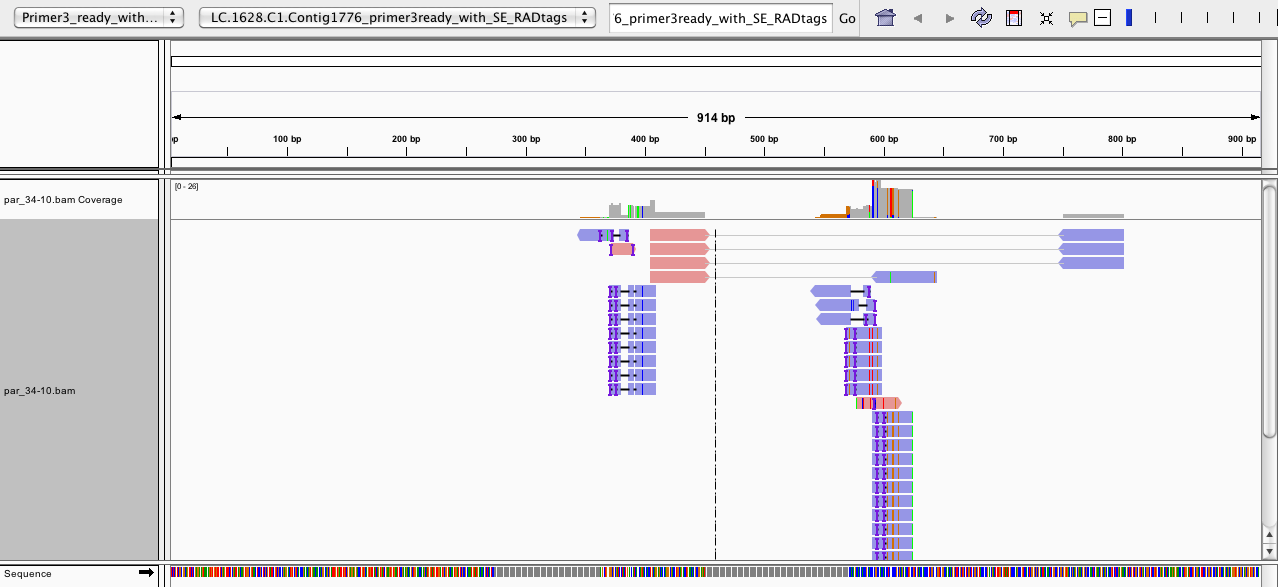
\includegraphics[width=\textwidth]{stampy_par_34-10_vs_primer3ready_igv}
\caption{Example read alignment of all standard RAD reads of individual par\_34-10 against one PE contig pair reference sequence.}
\label{stampy_par_34-10_vs_primer3ready_igv}
\end{figure}
%
\cite{Kosugi2013} have developed a few Perl scripts that deal with the problem of false positive alignments especially when doing a so-called \emph{targeted alignment}\footnote{when the reference sequence is much smaller than the source of the reads to be mapped} by removing reads that map with too many mismatches. They show that filtering by mapping quality score is rather ineffective when trying to improve a targeted alignment. Their programme \texttt{coval-refine} by default removes all reads with more than 2 \glspl{indel}, 1 indel and 1 soft-clipped end and 2 soft-clipped ends. I have changed \texttt{coval-refine} so that indels count like two mismatches. I have set the maximum proportion of mismatches to 0.1. Thus SE reads are 46 base pairs long and are allowed to have up to 5 mismatches. The 51 base pair long PE reads are also allowed up to 5 mismatches. By default, \texttt{coval-refine} counts ambiguous positions in the reference as mismatches. I therefore changed \texttt{coval-refine} to take correct account of the dual ambiguity codes RWYMKS. Figure \ref{coval-refine} shows the mapping result after \texttt{coval-refine} treatment for one individual and one reference sequence.
%
\begin{figure}
\centering
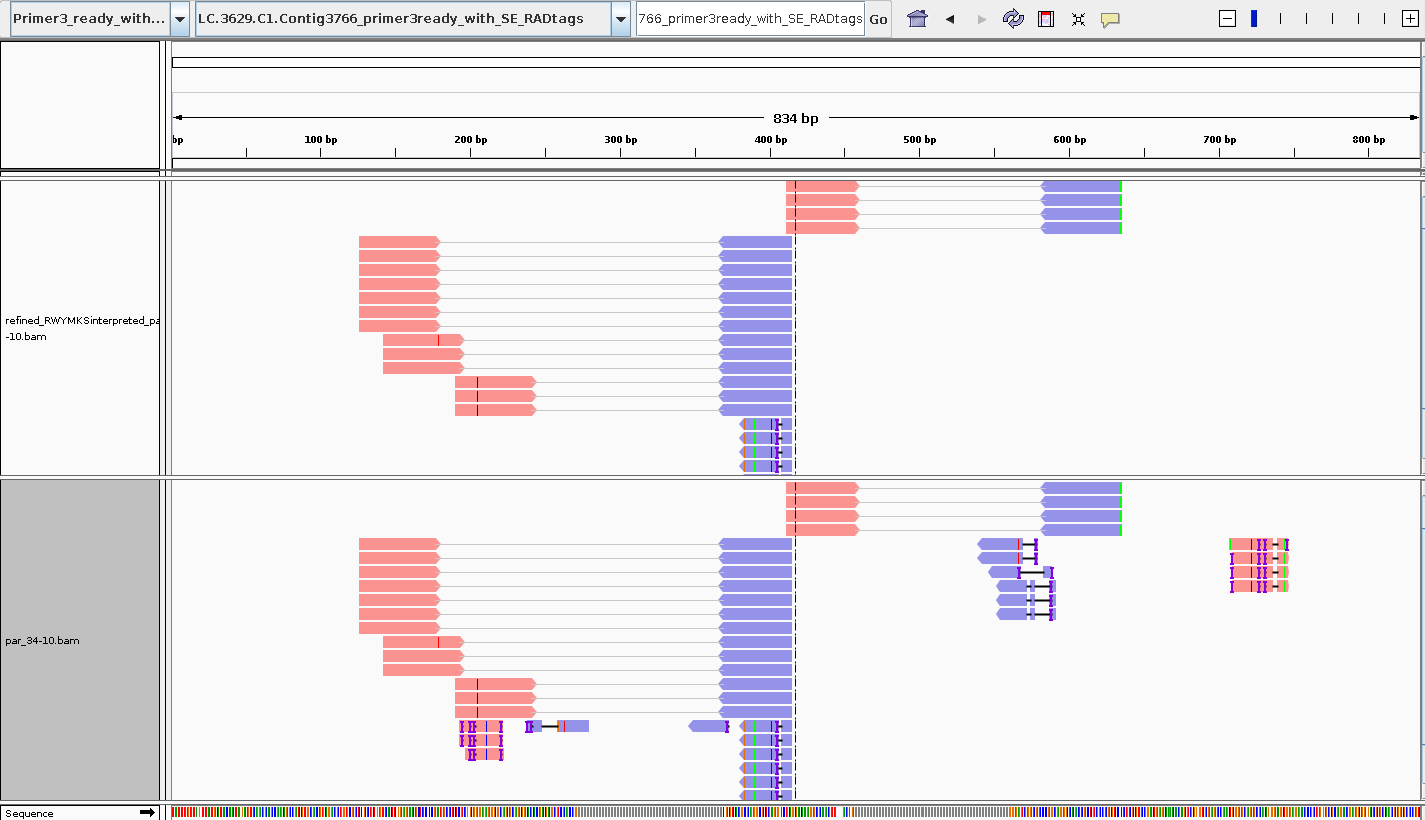
\includegraphics[width=\textwidth]{stampy_par_34-10_vs_primer3ready_after_coval-refine_igv}
\caption{Read alignment of all standard RAD reads of individual par\_34-10 against one PE contig pair consensus sequence. Upper track after \texttt{coval-refine} filtering. Lower track is without \texttt{coval-refine} filtering for comparison.}
\label{coval-refine}
\end{figure}
%

%
%
%

%% ---------------------------------------------------
\FloatBarrier
\subsection{Estimation of template amount for selective PCR}\label{ch:qPCR}
%% ---------------------------------------------------

I estimated the amount of template that went into the selective PCR for the SbfI$+$XhoI double-digest library (see figure \ref{ddRAD_protocol_overview}) with quantitative PCR \citep{Rutledge2003}.

I took an aliquot of the selective PCR product and determined its DNA concentration with picoGreen and a fluorometer\comment{probably 3 replicate measurements $\rightarrow$ lab book}. I made a serial dilution of 8 times 1:10 from this PCR product and used this to produce a standard curve. I created three replicates of the standard curve and three replicates of the target, i. e. the solution before selective PCR. The \gls{Ct} threshold was automatically set by the \textit{q}PCR machine and, except for the lowest template concentration of the standard dilution, the melting temperature of the PCR products were always very close to 79$^{\circ}$C. Assuming a mean template molecule length of 550 \gls{bp} and 16,000 loci from this double-digest library (see equation \ref{eq:exp_number_ddRAD_loci}), the \textit{q}PCR results indicate that on average only 1.26 ($\pm$ 0.37) template molecules per locus and individual went into the selective PCR\footnote{see DD\_RAD\_LIB\_101111\_data.xls}.


%% ------------------------------------------------------------------------------------------
\FloatBarrier
\subsection{comparison of different double-digest RAD protocols}
%% ------------------------------------------------------------------------------------------

Please see the table on the following page.\label{compProt}

\pagebreak

\begin{landscape}

\ctable[ 
	caption =  {comparison of different protocols for non-standard RAD$^{a}$ (see figure \ref{ddRAD_protocol_overview})},
	%label = compProt,
%	pos = t,
%	sideways,
	width = 240mm,
	captionskip = 1ex, % bring the caption closer to the table
	doinside=\scriptsize,
	center,
]
{l>{\raggedright}X>{\raggedright}X>{\raggedright}X>{\raggedright}X>{\raggedright}X>{\raggedright}X>{\raggedright}X}
{
\tnote[a]{\scriptsize without a random shearing step}
}
{
\FL
\textbf{protocol}   &   \textbf{adapters}   &   \textbf{DNA isolation}   &   \textbf{digestion}   &   \textbf{ligation}   &   \textbf{gel size selection}   &   \textbf{PCR}   &   \textbf{purification}
\ML
\cite{Peterson2012}		& P1 and P2 adapter at stock conc. of 40$\mu$M, short adapters and long PCR primers	& NA	& digest for 3h, no heat-inact. -- instead bead puri.	& 30min ligation at RT, 2-10 fold excess of adapters to sticky ends	& before PCR, automated DNA size selection with Pippin-Prep (Sage Science)	& 20ng size-selected library per PCR reaction, 2$\mu$M end conc. of each PCR primer, only 8-12 cycles (?!) 	& AMPure beads \NN % the ``\rowcolor'' command requires the ``colortbl'' package
\rowcolor[gray]{0.9} \cite{Andolfatto2011}		& 10$\mu$M stock conc., short adapters + long PCR primers	& Puregene (Qiagen)	& 10ng DNA per sample, with 3.3U of 4bp cutter MseI (i. e. no double-digerst), 3h at 37$^{\circ}$C followed by heat-inact.	& 5nmole adapters, only 1 U of T4 DNA ligase in a volume of 50$\mu$l, 1h at 16$^{\circ}$C 	& before PCR, ladder mixed into library, 2\% gel	& only 15 cycles, Phusion	& AMPure beads \NN
\cite{Parchman2012}		& 1$\mu$M stock conc. for P1 (EcoRI) adapter, 
					10$\mu$M stock conc. for P2 (MseI) adapter, 
					annealing in pure water (?!), 
					short adapters + long PCR primers	& NA	& 6- and 4bp cutter, 10U EcoRI, only 1U MseI, digestion in T4 buffer, 
														NaCl added to $\sim$50mM end conc.,
														volume 9$\mu$l, 8h, heat-inact.		& 1pmole EcoRI adapter, 10pmole MseI adapter, 
																						67 NEB units T4 ligase, 6h at 16$^{\circ}$C, 
																						ligation in only 11.4$\mu$l 				& after PCR, 2.5\% gel, low electric field gel runs,
																															EtBr gels, many lanes					&  \vspace{-8pt}{\color{red}individual PCR before pooling samples and before gel size selection},
																													   											30 cycles (?!), only 0.08$\mu$M end conc. of each primer in PCR (?!),
																																								BioRad Iproof High Fidelity DNA polymerase						& QiaQuick spin columns \NN
\rowcolor[gray]{0.9} this study & long adapters short PCR primers (fig. \ref{adapter_outline}) & silica spin columns (Qiagen)	& 132 ng per sample, 10 U/sample SbfI-HF, 20 U/sample XhoI	, NEBuffer 4, 3 h at 37$^{\circ}$C followed by heat-inact. &	$\sim$22 fold excess of adapters to sticky ends, 400 NEB U/sample ligase, 2 h at RT, then over night at 4$^{\circ}$C followed by heat-inact. &	before PCR, 1\% agarose gel with EtBr, whole pooled library in one lane, 13 V/cm &	20-24 cycles, Phusion Mastermix, 1.0$\mu$M of each thiol-protected primer & Qiagen MinElute spin columns \NN
\LL
}

\end{landscape}



%% ------------------------------------------------------------------------------------------
\FloatBarrier
\subsection{PCR duplicates in the standard SbfI RAD data}
%% ------------------------------------------------------------------------------------------

The standard SbfI RAD library had been sequenced on 4 lanes of an Illumina GAIIx sequencer with increasing template amount. I ran the programmes \texttt{RADpools} and \texttt{RADtags} from the \href{https://github.com/johnomics/RADtools.git}{\texttt{RADtools}} package version 1.2.1 on the raw data of these four lanes separately. \texttt{RADpools} demultiplexes reads by barcode, filters them according to base call quality scores and finally sorts read sequences alphabetically in individual read files. The programme \texttt{RADtags} then takes these sorted read files and calls \glspl{RAD tag} based on maximum pairwise mismatch counts. \texttt{RADtools} therefore uses alphabetical sorting of reads (within individuals) in order to reduce the number of pairwise mismatch counts it has to perform to call clusters of reads into \glspl{RAD tag}. This is obviously a suboptimal clustering strategy since it does not guarantee to cluster all similar sequences together. For each \gls{RAD tag} it reports the read count as well as \gls{fragment} count. Different fragments are recognised by different \gls{pe} reads, allowing for sequencing errors. PCR duplicates have the same PE read sequences and thus don't increase fragment count but do increase read count. I then ran my script \texttt{investigate\_PCR\_duplicates.pl} on the individual output files of \texttt{RADtags} from each lane in order to determine the total number of PCR duplicates from the read and fragment counts that it had put out for each cluster of \gls{se} reads. I then repeated the same analysis for all reads combined.

%% ------------------------------------------------------------------------------------------
\FloatBarrier
\subsection{Investigation of restriction enzyme recognition sequences within RAD reads}
%% ------------------------------------------------------------------------------------------


%%% -----------------------------------------------------------------------------
\subsubsection{SbfI and XhoI site frequency distributions}\label{site_frequency_distributions}
%%% -----------------------------------------------------------------------------

For the figures \ref{SbfI_frequency_dist_per_ind}, \ref{ddRAD_SbfI_frequency_dist} and \ref{ddRAD_XhoI_frequency_dist} I used my script \texttt{position.pl} to tally -- for each individual separately -- the positions in the \emph{unique} read sequences where an SbfI or XhoI recognition sequence was found. Each line in these plots connects the site frequencies of one individual. SE and PE reads were analysed separately. The reason for collapsing the reads into unique sequences is to remove the effect of PCR duplicates. Any peaks in the distributions can thus not be caused by PCR duplicates.

In figure \ref{SbfI_frequency_dist_per_ind} (a), there are three peaks in SbfI frequency at position 29, 34 and 39. Are these peaks caused by repetitive genome sequences that just happened to have an SbfI site at those positions? In order to investigate this, I used command line \ref{cmd:cluster_size_by_SbfI_position} in order to cluster all SbfI site containing reads from from the standard SbfI-RAD data set by the subsequence left (5') of their SbfI site.
%
\begin{cmd}
\captionsetup{type=cmd}
\begin{Verbatim}[fontsize=\scriptsize, formatcom=\color{darkgray}]

zcat *fq_1.gz | awk '(NR-2)%4==0' | grep "CCTGCAGG" | \
sort | uniq | cluster.pl > all_ind_pre_SbfI_cl_size_by_pos.cl
\end{Verbatim}
\caption{\small This command line clusters \texttt{uniq}-ed SE reads of all individuals that contain an SbfI site and then prints out foreach SbfI site position in the SE read length the cluster sizes that have been found. My custom script \texttt{cluster.pl} first groups reads by SbfI position and then clusters them within groups by mismatch count on the subsequence left of the SbfI site, thus ignoring the potentially non-homologous genomic sequence (due to religation) downstream of the SbfI site.}
\label{cmd:cluster_size_by_SbfI_position}
\end{cmd}
%
If the peaks at read position 29, 34 and 39 in figure \ref{SbfI_frequency_dist_per_ind} (a) were due to repetitive genome sequences, then the reads with SbfI sites at those positions should find themselves in bigger clusters than other reads.
%
\begin{figure}
\begin{knitrout}
\definecolor{shadecolor}{rgb}{0.969, 0.969, 0.969}\color{fgcolor}

{\centering \includegraphics[width=.9\linewidth]{figure/cluster_size_by_SbfI_position-1} 

}



\end{knitrout}
\caption{Cluster size for reads with different position of SbfI site in the SE reads of the standard SbfI-RAD library.}
\label{cluster_size_by_SbfI_position}
\end{figure}
%
Large cluster sizes are indeed found for reads with SbfI site at read position 29, 34 and 39 (figure \ref{cluster_size_by_SbfI_position}). This supports the idea, that the peaks of SbfI site frequency are caused by repetitive genome sequences that happen to have an SbfI site at these positions.

There are two individuals in figure \ref{SbfI_frequency_dist_per_ind} (b) which have exceptionally high SbfI site frequencies in PE reads (individual "ery\_30-8" and individual "ery\_30-17").
%
\begin{cmd}
\captionsetup{type=cmd} % this is necessary for the hyperlink to work, see manual for caption package, 6.5 about hyperref
\begin{Verbatim}[formatcom=\color{darkgray}, fontsize=\scriptsize]

paste <(zcat ery_30-8.fq_1.gz | awk '(NR-2)%4==0') <(zcat ery_30-8.fq_2.gz | \
awk '(NR-2)%4==0') | grep " .*CCTGCAGG" | sort | uniq -c | sort -nrk 1 | less -S
\end{Verbatim}
\caption{\small This command takes the SE and PE reads from one individual and pastes them side by side separated by a tab character. It then extracts those lines where the PE read contains an Sbf recognition sequence, counts the number of occurrences of identical lines and presents the most common lines at the top.}
\label{cmd:present_pair_with_SbfI}
\end{cmd}
%
The exceptionally high number of SbfI sites at the beginning of PE reads from these individuals can be explained by P1 adapter dimers and the fact that the barcode sequences for these two individuals (\texttt{GCGCC} and \texttt{TGACC}) end with \texttt{CC} and that these barcode sequences (or at least the \texttt{CC} part) appear at the beginning of PE reads into P1 adapters, thus recreating an SbfI recognition sequence (fig. \ref{SbfI_in_PE_reads_of_ery_30-8}). An equivalent but not as frequent pattern can be found in the reads of individual "par\_34-3", which has the barcode \texttt{AACCC}. The fact that the barcode sequence (or part of it) can be found at the beginning of PE reads can be explained by P1-P1 dimers where one of the adapters gets sheared off after (or within) the barcode sequence followed by ligation of the P2 adapter, which is necessary for illumina sequencing. 
%
\begin{figure}
%, frame=single, framesep=10pt, label=PE reads with SbfI site from ind. ery\_30-8]
\begin{Verbatim}[fontfamily=courier, fontsize=\tiny, commandchars=\\\{\}]
  count		SE reads					PE reads
    175 TGCA{\color{purple}GGCGC}{\color{orange}AGATCGGAAGAGCG}{\color{blue}GTTCAGCAGGAATGCCGAGACCG} {\color{purple}GCG}\underline{{\color{purple}CC}TGCA{\color{purple}GG}}{\color{purple}CGC}{\color{orange}AGATCGGAAGAGCG}{\color{teal}TCGTGTAGGGAAAGAGTGTAGAT}
     22 TGCAGG{\color{orange}AGATCGGAAGAGCG}{\color{blue}GTTCAGCAGGAATGCCGAGACCGAT}A \underline{CCTGCA{\color{purple}GG}}{\color{purple}CGC}{\color{orange}AGATCGGAAGAGCG}{\color{teal}TCGTGTAGGGAAAGAGTGTAGATCTC}
\end{Verbatim}
\caption{PE reads with SbfI site from ind. ery\_30-8. \emph{underlined}: SbfI recognition sequence; {\color{purple}\texttt{GCGCC}}: barcode sequence; {\color{orange}\texttt{AGA\ldots GCG}}: sequence common to P1 and P2 adapter; {\color{teal}\texttt{TCG}\ldots}: P1 adapter sequence; {\color{blue}\texttt{GTT}\ldots}: P2 adapter sequence. This figure was created from the output of command \ref{cmd:present_pair_with_SbfI}.}
\label{SbfI_in_PE_reads_of_ery_30-8}
\end{figure}
%
The overall higher frequency of SbfI sites in PE reads of these three individuals (figure \ref{relative_SbfI_frequencies}) can be explained by reads into the P1 adapter, i. e. sequencing the recreated SbfI site (figure \ref{par_34-3_SbfI_PE_read_into_P1}).
%
\begin{figure}
\begin{knitrout}
\definecolor{shadecolor}{rgb}{0.969, 0.969, 0.969}\color{fgcolor}

{\centering \includegraphics[width=.9\linewidth]{figure/relative_SbfI_frequencies-1} 

}



\end{knitrout}
\caption{SbfI site frequency distributions in uniqued PE reads for each individual relative to its read count (after quality filtering with \texttt{process\_radtags}). The three individuals with barcodes ending in \texttt{CC} are highlighted with different colours.}
\label{relative_SbfI_frequencies}
\end{figure}
%
\begin{cmd}
\captionsetup{type=cmd}
\begin{Verbatim}[fontsize=\scriptsize, formatcom=\color{darkgray}]

paste <(zcat par_34-3.fq_1.gz | awk '(NR-2)%4==0') <(zcat par_34-3.fq_2.gz | \
awk '(NR-2)%4==0') | grep "CCTGCAGG.*AGATCGGA" | sort -k 2 | uniq | vim -
\end{Verbatim}
\caption{\small This command is similar to command \ref{cmd:present_pair_with_SbfI}. However, in addition to the SbfI recognition sequence it extracts lines that contain an 8 base pair sequence from the beginning of the illumina adapters (see figure \ref{adapter_outline}).}
\label{cmd:read_into_P1_detection}
\end{cmd}
%
\begin{figure}
\centering
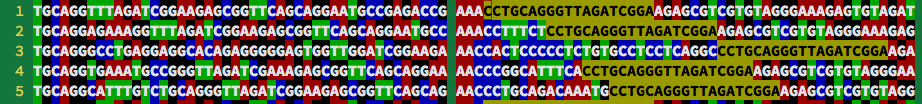
\includegraphics[width=\textwidth]{par_34-3_SbfI_PE_read_into_P1}
\caption{Snapshot from the output of command \ref{cmd:read_into_P1_detection}. The highlighted subsequences contain the SbfI recognition sequence overlapping with the reverse complement of the barcode sequence \texttt{AACCC} and the beginning of the P1 adapter sequence. The subsequences left of the SbfI sequence in the PE reads are genomic. Note that these genomic sequences can also be found in the corresponding SE reads (after reverse-complementing) right after the remainder of the SbfI sites at the beginning of the SE reads.}
\label{par_34-3_SbfI_PE_read_into_P1}
\end{figure}

The reads for figure \ref{ddRAD_SbfI_frequency_dist} and \ref{ddRAD_XhoI_frequency_dist} are from reads of the SbfI$+$XhoI double-digest RAD library and were quality filtered with \texttt{stacks}' \texttt{process\_radtags} and my custom script \texttt{grep\_true\_RADtag.pl}. In contrast to figure \ref{SbfI_frequency_dist_per_ind}, the SbfI and XhoI site frequencies in these two figures are expressed in relation to the individual's read count, thus removing the effect of inter-individual variation in read count on the site frequency distributions.

The most striking pattern are the three outlier individuals for the PE reads containing SbfI sites in figure \ref{ddRAD_SbfI_frequency_dist}. The outlier individuals are "par\_34-3", "ery\_30-18" and "par\_34-14". This high relative frequency is not due to low read counts.
%
\begin{center}
\begin{tabular}{lr}
\toprule
sample ID & barcode\\
\midrule
34-3 & AACCC  \\
34-14 & GCGCC  \\
30-18 & TGACC  \\
\bottomrule
\end{tabular}
\end{center}
%
However, these three individuals are the only three whose barcode ends with \texttt{CC}. When looking at the output of the following command line, it becomes clear that the high frequencies of reads with SbfI sites from these three individuals is caused by reads into the P1 adapter, their barcode regenerating the SbfI recognition sequence.
%
\begin{Verbatim}[formatcom=\color{darkgray}, fontsize=\scriptsize]
awk '(NR-2)%4==0' par_34-3_cleaned_trueTags.fq_2 | \
grep CCTGCAGG | sort | uniq | cluster.pl > par_34-3_SbfI_PE.cl
\end{Verbatim}
%
The extreme similarity of the curves for these three individuals is also striking. This might be caused by common repetitive sequences containing two SbfI sites in close proximity.

Figure \ref{ddRAD_XhoI_frequency_dist} shows the XhoI site frequency distribution over SE and PE reads. There are no outlier individuals but clear common peaks of XhoI frequency at certain positions in the reads. I clustered all XhoI site containing SE reads by the subsequence left (5') of their XhoI site with my script \texttt{cluster.pl} and command \ref{cmd:cluster_size_by_XhoI_position}. 
%
\begin{cmd}
\captionsetup{type=cmd}
\begin{Verbatim}[fontsize=\scriptsize, formatcom=\color{darkgray}]

cat *cleaned_trueTags.fq_1 | awk '(NR-2)%4==0' | grep "CTCGAG" | \
sort | uniq | cluster.pl > all_ind_XhoI_in_SE_cl_by_pos.csv & 
\end{Verbatim}
\caption{\small This command is analogous to command \ref{cmd:cluster_size_by_SbfI_position}. It clusters \texttt{uniq}-ued SE reads of all individuals that contain an XhoI site and then foreach XhoI site position in the SE read length prints out the cluster sizes that have been found. My custom script \texttt{cluster.pl} first groups reads by XhoI position and then clusters them within groups by mismatch count on the subsequence left of the XhoI site, thus ignoring the potentially non-homologous genomic sequence (due to religation) downstream of the XhoI site.}
\label{cmd:cluster_size_by_XhoI_position}
\end{cmd}
%
Figure \ref{cluster_size_by_XhoI_position} shows for the SE reads that most of these peaks are the result of repetitive sequences since they coincide with large cluster sizes. 
%
\begin{figure}
\begin{knitrout}
\definecolor{shadecolor}{rgb}{0.969, 0.969, 0.969}\color{fgcolor}

{\centering \includegraphics[width=.9\linewidth]{figure/cluster_size_by_XhoI_position-1} 

}



\end{knitrout}
\caption{XhoI site frequency distribution for all uniqued SE reads together (red) and the corresponding sizes of clusters in which these reads find themselves (green).}
\label{cluster_size_by_XhoI_position}
\end{figure}
%



%%% -----------------------------------------------------------------------------
\subsubsection{Cluster Analysis}\label{cluster_analysis}
%%% -----------------------------------------------------------------------------

For the cluster analysis of genomic religation versus incomplete digestion, I have first collected all read pairs containing a restriction site from each individual with my script \texttt{grep\_fq\_read\_pairs.pl}. I have then used command \ref{cmd:cluster_SbfI_reads} with my script \texttt{cluster.pl} in order to cluster these reads by similarity of the subsequence left (5') of the restriction site. 
%
\begin{cmd}
\captionsetup{type=cmd}
\begin{Verbatim}[fontsize=\scriptsize, formatcom=\color{darkgray}]
paste <(awk '(NR-2)%4==0' *SbfI_reads.fq_1) <(awk '(NR-2)%4==0' *SbfI_reads.fq_2) | \
grep "CCTGCAGG" | sort | uniq | cluster.pl > all_uniq_SbfI_reads_clustered.cl
\end{Verbatim}
\caption{\small This command first pastes read pairs that contain SbfI sites sites side by side (SE left, PE right), then removes exact duplicate lines before clustering read pairs by the subsequence left of the SbfI site.}
\label{cmd:cluster_SbfI_reads}
\end{cmd}
%
I have used command \ref{cmd:cluster_size_by_XhoI_position} to cluster SE reads with SbfI or XhoI sites from the double-digest RAD library. In addition to cluster sizes, the script \texttt{cluster.pl} can also be set to print out the clusters themselves. The output file with clusters is then opened in the text editor VIM and the DNA sequences are highlighted with colours by a VIM plugin of \href{https://www.abc.se/~nylander/}{Johan Nylander}.

%%% -----------------------------------------------------------------------------
\FloatBarrier
\subsubsection{Read pair mapping analysis}\label{read_pair_mapping_analysis}
%%% -----------------------------------------------------------------------------

\paragraph{Quasi-random read pairs} 
With command \ref{cmd:extract_random_read_pairs} I have taken the 200,001st to 300,000th read pair from each individual in the standard RAD data set.
%
\begin{cmd}
\captionsetup{type=cmd}
\begin{Verbatim}[fontsize=\scriptsize, formatcom=\color{darkgray}]

for i in ../*fq_[12].gz; do (head -n 1200000 <(zcat $i) | \
tail -n 400000 > `basename $i .gz`.random)& done
\end{Verbatim}
\caption{\small This command line extracts the third set of 100,000 \href{http://en.wikipedia.org/wiki/FASTQ_format}{FASTQ} records from each read file.}
\label{cmd:extract_random_read_pairs}
\end{cmd}
%
For the SbfI$+$XhoI double-digest RAD data set I have used a very similar command, but extracted only the SE reads. All reads had passed my quality filtering steps\comment{I need to add description of quality filtering the raw read data}.

%
%
%

\paragraph{Bowtie2}
For the standard RAD library, I ran \texttt{bowtie2} with a maximum allowed fragment/insert size for a "valid paired alignment"\footnote{presumably synonymous to \gls{proper pair}} (\texttt{-X}) of 900. The upper end of gel size selection was at around 800 base pair fragment length (including Illumina adapters). For the read pair data from digital digestion,  I have set the maximum fragment/insert size to 120. The length of the original SbfI$+$XhoI SE reads was 96 \glspl{bp}. For both types of read pairs I ran \texttt{bowtie2} in \texttt{--very-sensitive-local} mode.

%
%
%

\paragraph{Counting \gls{concordant} read pairs}
I then extracted all reads from read pairs where both reads mapped, \gls{concordant}ly or not and disregarding mapping quality, sorted on names (both done as in command \ref{cmd:extract_sort_mapping_read_pairs}) and concatenated the individual sorted BAM files into one with \texttt{samtools cat}.
%
\begin{cmd}
\captionsetup{type=cmd}
\begin{Verbatim}[fontsize=\scriptsize, commandchars=\\\{\}]
parallel -j 5 'samtools view -\textcolor{red}{h}uF12 \{\} | \\
samtools sort -n -o \{.\}_F12_sort.bam -T \{.\} -' ::: *sam &
\end{Verbatim}
\caption{\small This command line extracts from each individual read mapping output file (in \gls{SAM} format) those read pairs where both reads mapped (\texttt{-F12}) and then sorts these SAM records by read name, which is necessary for concatenating the individual files into one with \texttt{samtools cat}.}
\label{cmd:extract_sort_mapping_read_pairs}
\end{cmd}
%
I then used command \ref{cmd:count_all_read_pairs} in order to count the total number of read pairs.
%
\begin{cmd}
\captionsetup{type=cmd}
\begin{Verbatim}[fontsize=\scriptsize, formatcom=\color{darkgray}]

samtools view -f64 all_random_F12_sort.bam | wc -l
\end{Verbatim}
\caption{\small This command line counts the number of SE reads (first in pair) in a mapping output file (binary \gls{SAM} format).}
\label{cmd:count_all_read_pairs}
\end{cmd}
%
Although, \texttt{bowtie2} reports a number of \gls{concordant}ly mapped read pairs in its mapping summary report, I have found that the \gls{proper pair} bit in the \href{http://samtools.github.io/hts-specs/SAMv1.pdf}{SAM flag} of each read record is not always set correctly. This seems to be linked to the inference of fragment/insert size, i. e. the length of the genomic fragment from which the SE read and the PE read is produced. I have therefore applied my own filtering to count \glspl{proper pair} (command \ref{cmd:count_genuine_proper_pairs}).
%
\begin{cmd}
\captionsetup{type=cmd}
\begin{Verbatim}[fontsize=\scriptsize, formatcom=\color{darkgray}, numbers=left]
samtools view -f2 -f16 -F32 all_random_F12_sort.bam | \
awk '$7 ~ "="' | \
awk '$4 > $8' | \
Isize.pl | \
awk '$10 < 900 && $10 > 50' | \
wc -l 
\end{Verbatim}
\caption{
\small This command line counts the number of genuinely \gls{concordant} read pairs in a mapping output file by applying a sequence of filters. The first line extracts all reverse mapping reads (\texttt{-f16}) whose mate did not map as reverse-complement (\texttt{-F32}) and which have the proper pair SAM flag bit set (\texttt{-f2}). The second line makes sure that both reads in the pair got mapped to the same reference contig. The third line makes sure that the reverse mapping read has a higher mapping position than its forward mapping mate (no dovetailing). The fourth line uses my custom script \texttt{Isize.pl} in order to calculate the fragment/insert size and the fifth line makes sure that the insert size is within the bounds of 50 and 900.
}
\label{cmd:count_genuine_proper_pairs}
\end{cmd}
%
My script \texttt{Isize.pl} calculates the insert/fragment size, also known as \emph{template length}, from the reported mapping positions of the read pair and the \href{http://samtools.github.io/hts-specs/SAMv1.pdf}{CIGAR} string of the reverse mapping read in the pair. It does this by adding up the matching bases reported in the CIGAR string of the reverse mapping read in order to add this to its reported mapping position\footnote{this results in the reference coordinate of the position right of the rightmost mapping base with respect to the reference sequence} and then subtracts from the result the reported mapping position of its forward mapping mate.\todo{include a drawing here, use tikz package}~Thus soft-clipped bases are not included in the calculated insert size.
%
\renewcommand{\epigraphflush}{center}
\setlength{\epigraphwidth}{.9\textwidth}
\setlength{\epigraphrule}{0pt}
%
{\mdseries
\epigraph{
A mapped base is a base in the read that corresponds one-to-one to a base in the reference.  So soft-clipped, hard-clipped, inserted and deleted bases are not mapped bases in that sense.
}
{Tim Fennell on the \href{http://sourceforge.net/p/samtools/mailman/message/28656712/}{\texttt{samtools} mailing list} on SourceForge}
%
\epigraph{
If all segments [reads] are mapped to the same reference, the unsigned [absolute] observed template length equals the number of bases from the leftmost mapped base to the rightmost mapped base.
}
{\cite{SAMformatSpec2011}}
}
%
I have also searched among the read pairs, which did not get the \gls{proper pair} bit set by \texttt{bowtie2}, for read pairs which still fulfill the criteria of proper pairs (command \ref{cmd:count_proper_pairs_without_flag_bit}).
%
\begin{cmd}
\captionsetup{type=cmd}
\begin{Verbatim}[fontsize=\scriptsize, formatcom=\color{darkgray}, numbers=left]
samtools view -F2 -f16 -F32 all_mapped_read_pairs_F12.bam | \
awk '$7 ~ "="' | \
awk '$4 > $8' | \
Isize.pl | \
awk '$10 < 900 && $10 > 50' | \
wc -l
\end{Verbatim}
\caption{\small This command line applies the same filters as command \ref{cmd:count_genuine_proper_pairs} to read pairs which did not get the \gls{proper pair} SAM flag bit set (\texttt{-F2}).}
\label{cmd:count_proper_pairs_without_flag_bit}
\end{cmd}
%
For the read pairs from digital digestion I used the same three commands (\ref{cmd:count_all_read_pairs} till \ref{cmd:count_proper_pairs_without_flag_bit}) as for the standard SbfI RAD read pairs, except for applying an accepted insert size range of 30 to 120.




%%% ---------------------------------------------------
%\section{Estimating divergence time of the two subspecies}
%%% ---------------------------------------------------
%
%\begin{itemize}
%\item work off questions
%\item leave details including command lines for suppl. material
%\item template amount estimation with fluorometer before and after PCR, qPCR
%\item how much heterozygosity within populations, after long distance dispersal
%\item leap-frog dispersal
%\item Lunt, Cooper, Cpn1, mitochondria
%\item ABS, simCoal
%\item long dispersal tail --> potential for contact between distal populations
%\item test gene flow <-> no gene flow model
%\item filtering paralogs in highly repetitive genomes
%\item large genome size $+$ genome size variation
%\item clustering algorithms: DNAclust, CD-Hit, afcluster, ustacks, starcode, UNEAK
%\end{itemize}
%
%
%\section{Results}
%
%\section{Interpretation of Results}
%
%
%
%% ********************************************************
%And now I begin my third chapter here \dots
%
%\cite{Baird2008} were the first to publish about RAD. \SI{12,3}{\micro\metre}
%
%Fig.~\vref{fragments-mapped-per-ind} shows the number of \glspl{fragment} mapped per individual.
%I am trying to find \glspl{snp} among individuals of the sample.
%% ********************************************************
%
%
%
%
%
%
%
%\subsection{First subsection in the first section}
%\dots and some more 
%
%\subsection{Second subsection in the first section}
%\dots and some more \dots
%
%\subsubsection{First subsub section in the second subsection}
%\dots and some more in the first subsub section otherwise it all looks the same
%doesn't it? well we can add some text to it \dots
%
%\subsection{Third subsection in the first section}
%\dots and some more \dots
%
%\subsubsection{First subsub section in the third subsection}
%\dots and some more in the first subsub section otherwise it all looks the same
%doesn't it? well we can add some text to it and some more and some more and
%some more and some more and some more and some more and some more \dots
%
%\subsubsection{Second subsub section in the third subsection}
%\dots and some more in the first subsub section otherwise it all looks the same
%doesn't it? well we can add some text to it \dots
%
%\section{Second section of the third chapter}
%and here I write more \dots
%
%\section{The layout of formal tables}
%This section has been modified from ``Publication quality tables in \LaTeX*''
% by Simon Fear.
%
%The layout of a table has been established over centuries of experience and 
%should only be altered in extraordinary circumstances. 
%
%When formatting a table, remember two simple guidelines at all times:
%
%\begin{enumerate}
%  \item Never, ever use vertical rules (lines).
%  \item Never use double rules.
%\end{enumerate}
%
%These guidelines may seem extreme but I have
%never found a good argument in favour of breaking them. For
%example, if you feel that the information in the left half of
%a table is so different from that on the right that it needs
%to be separated by a vertical line, then you should use two
%tables instead. Not everyone follows the second guideline:
%
%There are three further guidelines worth mentioning here as they
%are generally not known outside the circle of professional
%typesetters and subeditors:
%
%\begin{enumerate}\setcounter{enumi}{2}
%  \item Put the units in the column heading (not in the body of
%          the table).
%  \item Always precede a decimal point by a digit; thus 0.1
%      {\em not} just .1.
%  \item Do not use `ditto' signs or any other such convention to
%      repeat a previous value. In many circumstances a blank
%      will serve just as well. If it won't, then repeat the value.
%\end{enumerate}
%
%A frequently seen mistake is to use `\textbackslash begin\{center\}' \dots `\textbackslash end\{center\}' inside a figure or table environment. This center environment can cause additional vertical space. If you want to avoid that just use `\textbackslash centering'
%
%
%\begin{table}
%\caption{A badly formatted table}
%\centering
%\label{table:bad_table}
%\begin{tabular}{|l|c|c|c|c|}
%\hline 
%& \multicolumn{2}{c}{Species I} & \multicolumn{2}{c|}{Species II} \\ 
%\hline
%Dental measurement  & mean & SD  & mean & SD  \\ \hline 
%\hline
%I1MD & 6.23 & 0.91 & 5.2  & 0.7  \\
%\hline 
%I1LL & 7.48 & 0.56 & 8.7  & 0.71 \\
%\hline 
%I2MD & 3.99 & 0.63 & 4.22 & 0.54 \\
%\hline 
%I2LL & 6.81 & 0.02 & 6.66 & 0.01 \\
%\hline 
%CMD & 13.47 & 0.09 & 10.55 & 0.05 \\
%\hline 
%CBL & 11.88 & 0.05 & 13.11 & 0.04\\ 
%\hline 
%\end{tabular}
%\end{table}
%
%\begin{table}
%\caption{A nice looking table}
%\centering
%\label{table:nice_table}
%\begin{tabular}{l c c c c}
%\hline 
%\multirow{2}{*}{Dental measurement} & \multicolumn{2}{c}{Species I} & \multicolumn{2}{c}{Species II} \\ 
%\cline{2-5}
%  & mean & SD  & mean & SD  \\ 
%\hline
%I1MD & 6.23 & 0.91 & 5.2  & 0.7  \\
%
%I1LL & 7.48 & 0.56 & 8.7  & 0.71 \\
%
%I2MD & 3.99 & 0.63 & 4.22 & 0.54 \\
%
%I2LL & 6.81 & 0.02 & 6.66 & 0.01 \\
%
%CMD & 13.47 & 0.09 & 10.55 & 0.05 \\
%
%CBL & 11.88 & 0.05 & 13.11 & 0.04\\ 
%\hline 
%\end{tabular}
%\end{table}
%
%
%\begin{table}
%\caption{Even better looking table using booktabs}
%\centering
%\label{table:good_table}
%\begin{tabular}{l c c c c}
%\toprule
%\multirow{2}{*}{Dental measurement} & \multicolumn{2}{c}{Species I} & \multicolumn{2}{c}{Species II} \\ 
%\cmidrule{2-5}
%  & mean & SD  & mean & SD  \\ 
%\midrule
%I1MD & 6.23 & 0.91 & 5.2  & 0.7  \\
%
%I1LL & 7.48 & 0.56 & 8.7  & 0.71 \\
%
%I2MD & 3.99 & 0.63 & 4.22 & 0.54 \\
%
%I2LL & 6.81 & 0.02 & 6.66 & 0.01 \\
%
%CMD & 13.47 & 0.09 & 10.55 & 0.05 \\
%
%CBL & 11.88 & 0.05 & 13.11 & 0.04\\ 
%\bottomrule
%\end{tabular}
%\end{table}

%----------------------------
% Bibliography
%----------------------------

\bibliographystyle{elsarticle-harv}
\bibliography{/Users/Claudius/Documents/MyLiterature/Literature}
%
\end{document}
